\documentclass[aspectratio=169]{beamer}

\usepackage[export]{adjustbox}
\usepackage[many]{tcolorbox}
\usepackage{mathrsfs,amsmath}
\usepackage{tikz}
\usepackage{physics}
\usepackage[ngerman]{babel}

\title{Fourier Transformation}
\subtitle{und ihre Anwendungen}
\author{Elias Kiene, Marek Freunscht}
\date{\today}

\begin{document}

\begin{frame}
    \titlepage
\end{frame}

\begin{frame}
    \frametitle{Themen}
    \begin{enumerate}
        \item Fourier Reihen
        \item Was ist eine Fourier Transformation?
        \item Herleitung der Fourier Transformation
        \item Inverse Fourier Transformation
        \item Diskrete Fourier Transformation
        \item Anwendungen
    \end{enumerate}
\end{frame}
	
	\begin{frame}
	\frametitle{Fourier Reihe}
	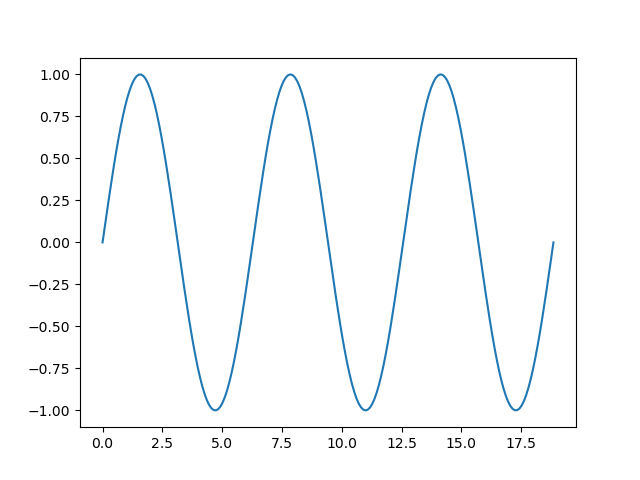
\includegraphics[width=200px]{images/00-rect-0.png}
\end{frame}

\begin{frame}
	\frametitle{Fourier Reihe}
	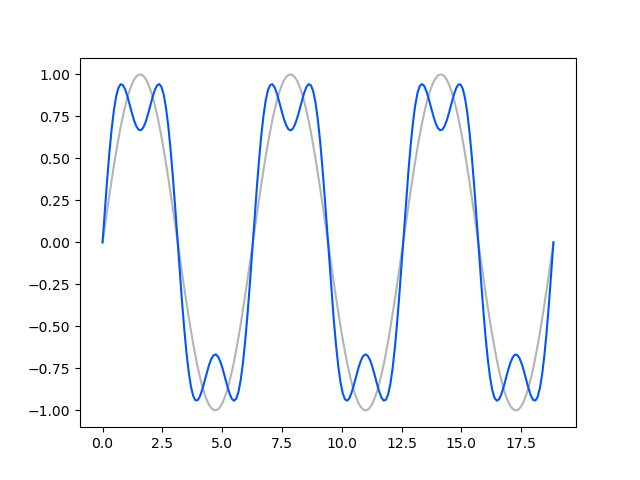
\includegraphics[width=200px]{images/00-rect-1.png}
\end{frame}

\begin{frame}
	\frametitle{Fourier Reihe}
	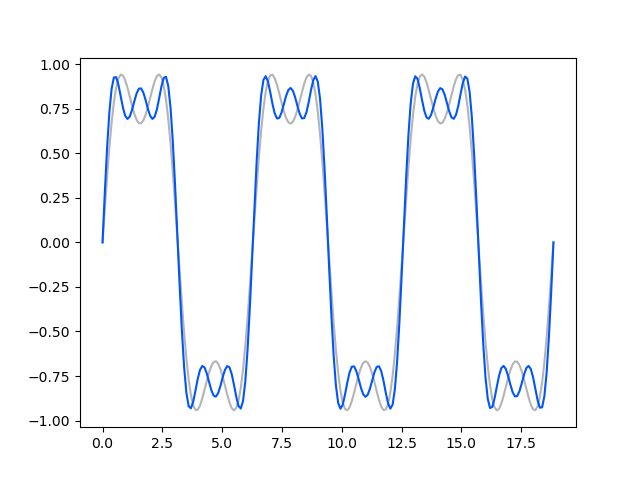
\includegraphics[width=200px]{images/00-rect-2.png}
\end{frame}

\begin{frame}
	\frametitle{Fourier Reihe}
	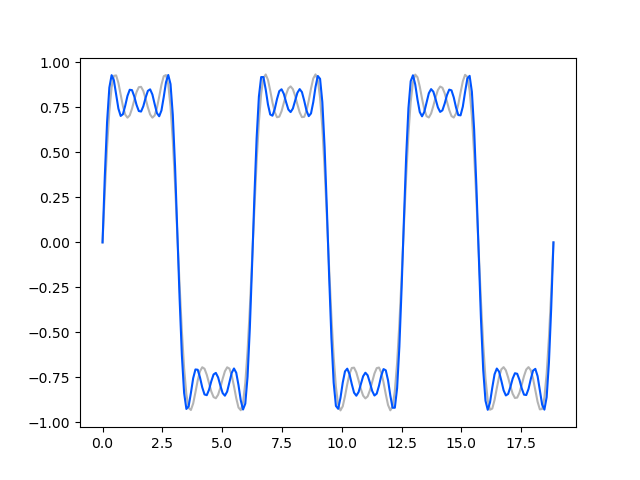
\includegraphics[width=200px]{images/00-rect-3.png}
\end{frame}

\begin{frame}
	\frametitle{Fourier Reihe}
	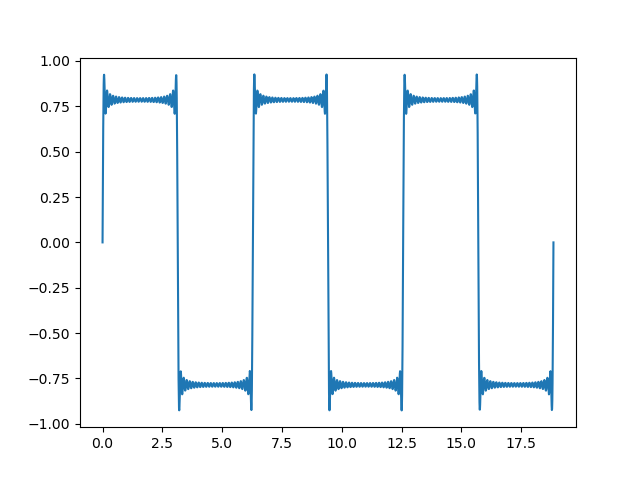
\includegraphics[width=200px]{images/00-rect-4.png}
\end{frame}

\begin{frame}
	\frametitle{Fourier Reihe}
	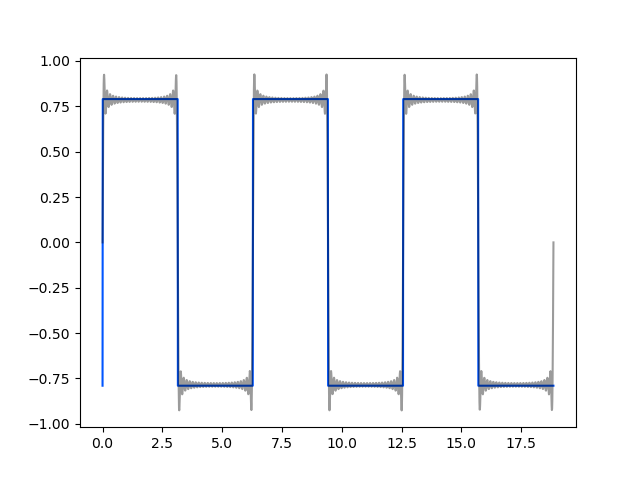
\includegraphics[width=200px]{images/00-rect-5.png}
\end{frame}

\begin{frame}
	\frametitle{Fourier Reihe}
	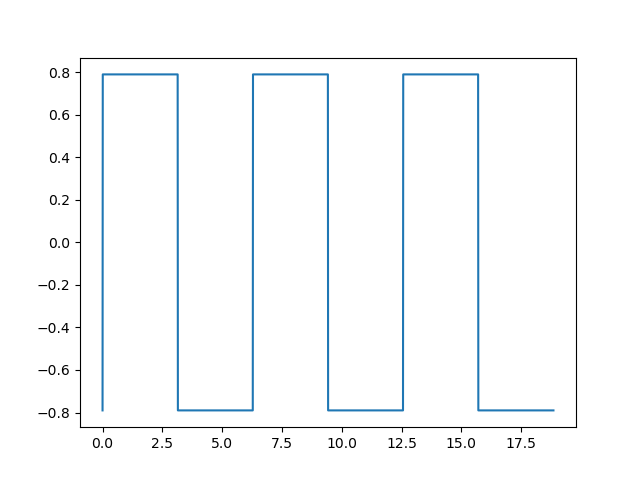
\includegraphics[width=200px]{images/00-rect-6.png}
	\begin{align}
		\sum_{k=1,3,5,\cdots}^{\infty}\frac{sin(kx)}{k}
	\end{align}
\end{frame}

\begin{frame}
	\frametitle{Fourier Reihe}
	\begin{itemize}
		\item Periodische Signale können durch Summen von Sinus- und Kosinuswellen approximiert werden
		\item Hierbei werden diese in eine Grundschwingung und Oberschwingungen mit ganzzahligen Vielfachen der Grundfrequenz aufgeteilt
		\item $f(t) = \displaystyle\frac{a_0}{2} + \displaystyle \sum_{k=1}^{\infty}\left[a_k cos(\omega_0 kt) + b_k sin(\omega_0 kt)\right]$
	\end{itemize}
\end{frame}

\begin{frame}
	\frametitle{Wieso Sinus und Kosinus}
	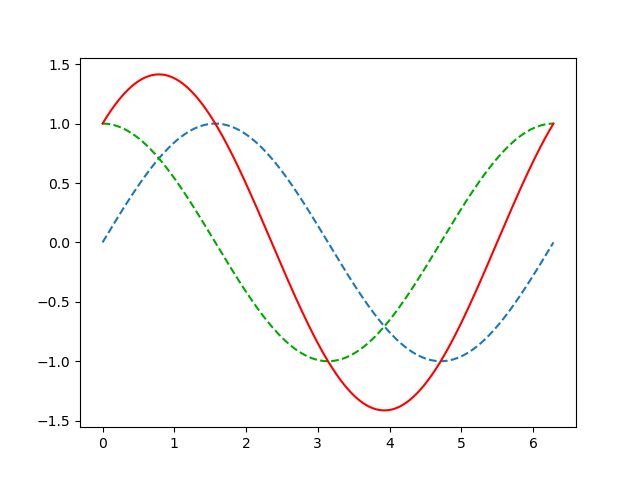
\includegraphics[width=200px]{images/00-sincos.png}
	\begin{itemize}
		\item Sinus ist punktsymmetrisch
		\item Kosinus ist achsensymmetrisch
		\item Phasenverschiebung durch Sinus-Kosinus Kombination
	\end{itemize}
\end{frame}

\begin{frame}
	\frametitle{Oberwellen}
	\begin{columns}
		\begin{column}{0.5\linewidth}
			\centering
			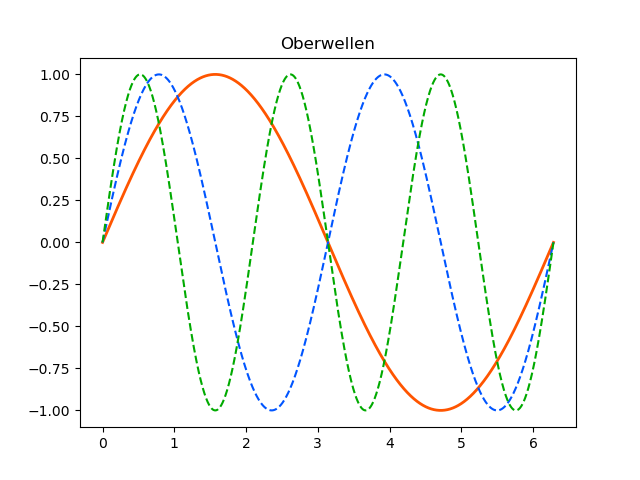
\includegraphics[width=170px]{images/00-oberwellen-0.png}
			Bei $\omega_k = n\,\omega_0$ wird die Grundfrequenz nicht beeinflusst.
		\end{column}
		\begin{column}{0.5\linewidth}
			\centering
			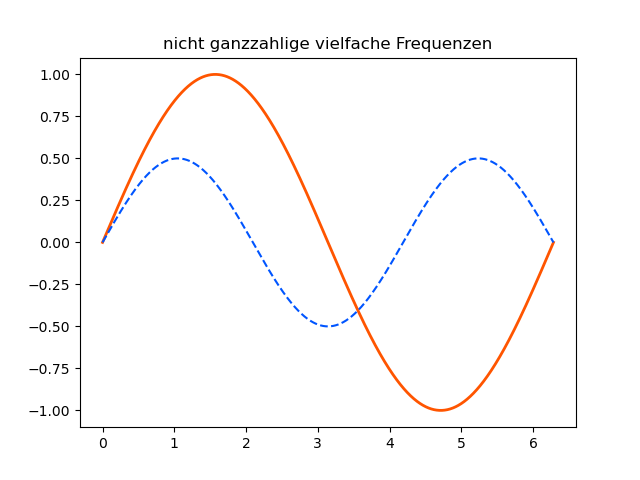
\includegraphics[width=170px]{images/00-oberwellen-1.png}
			Andere Frequenzen beeinflussen die Grundfrequenz der Schwingung
		\end{column}
	\end{columns}
\end{frame}

\begin{frame}
	\frametitle{Oberwellen}
	\begin{columns}
		\begin{column}{0.5\linewidth}
			\centering
			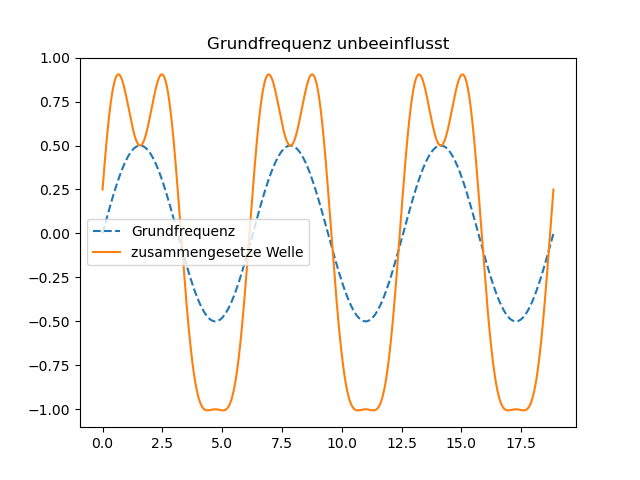
\includegraphics[width=170px]{images/00-oberwellen-zus-0.png}
			$sin(x) + \frac{cos(2x)}{4}+\frac{sin(3x)}{4}$
		\end{column}
		\begin{column}{0.5\linewidth}
			\centering
			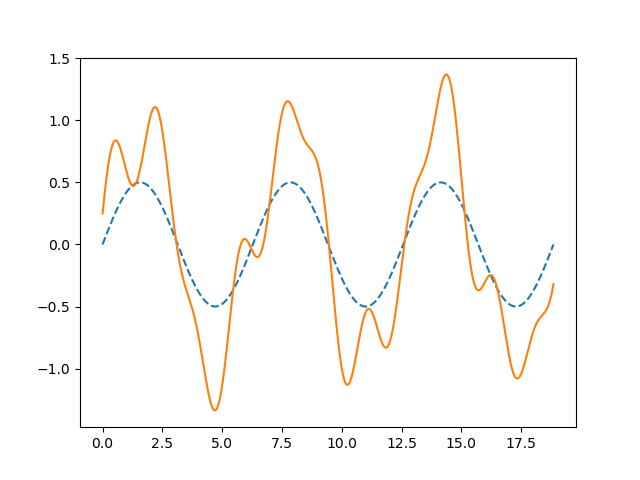
\includegraphics[width=170px]{images/00-oberwellen-zus-1.png}
			$sin(x) + \frac{cos(2.23x)}{4}+\frac{sin(3.56x)}{4}$
		\end{column}
	\end{columns}
\end{frame}

\begin{frame}
	\frametitle{Wie werden die Fourier Koeffizienten gewählt?}
\end{frame}

\begin{frame}
	\frametitle{Komplexe Darstellung der Fourierreihe}
	HIER MAREKS FOLIEN REIN !!!111!
\end{frame}

\begin{frame}
	\frametitle{Herleitung komplexe Darstellung}
	Komplexe Darstellung von Sinus und Kosinus:
	\begin{align*}
		cos(\varphi) &= \frac{e^{i\varphi}+e^{-i\varphi}}{2} \\
		sin(\varphi) &= \frac{e^{i\varphi}-e^{-i\varphi}}{2i}
	\end{align*}
\end{frame}
\begin{frame}
	\frametitle{Herleitung komplexe Darstellung}
	\begin{align*}
		f(t) &= \sum_{k=0}^{\infty}\left[a_k cos(kt) + b_k sin(kt)\right] \\
		&= \sum_{k=0}^{\infty}\left[a_k \frac{e^{ikt}+e^{-ikt}}{2} + b_k \frac{e^{ikt}-e^{-ikt}}{2i}\right] \\
		&= \sum_{k=0}^{\infty}\left[\frac{a_k}{2}e^{ikt} + \frac{a_k}{2}e^{-ikt} + \frac{b_k}{2i}e^{ikt} - \frac{b_k}{2i}e^{-ikt}\right] \\
		&= \sum_{k=0}^{\infty}\left[\frac{1}{2}\left(a_k-b_ki\right)e^{ikt} + \frac{1}{2}\left(a_k+b_ki\right)e^{-ikt}\right] \\
		&= \sum_{k=0}^{\infty}\left[\frac{1}{2}\left(a_k-b_ki\right)e^{ikt}\right] + \sum_{k=0}^{\infty}\left[\frac{1}{2}\left(a_k+b_ki\right)e^{-ikt}\right] \\
	\end{align*}
\end{frame}

\begin{frame}
	\frametitle{Herleitung komplexe Darstellung}
	\begin{align*}
		f(t) &= \sum_{k=0}^{\infty}\left[\frac{1}{2}\left(a_k-b_ki\right)e^{ikt}\right] + \sum_{k=0}^{\infty}\left[\frac{1}{2}\left(a_k+b_ki\right)e^{-ikt}\right] \\ \\
		Sei \,\,\, &\,c_k = \begin{cases}
			\,\,\displaystyle\frac{1}{2}(a_k - b_ki) \quad f\ddot{u}r\,\,\, k > 0 \\ \\
			\,\,\displaystyle\frac{1}{2}(a_k + b_ki) \quad f\ddot{u}r\,\,\, k \le 0 
		\end{cases} \\ \\
	f(t) &= \sum_{k=-\infty}^{\infty}c_k e^{ikt}
	\end{align*}
\end{frame}

\begin{frame}
	\frametitle{Berechnung der komplexen Koeffizienten}
	\begin{align*}
		\int_{0}^{T}f(t) e^{-imt}
		&= \int_{0}^{T} \left(\sum_{k=-\infty}^{\infty}c_k e^{ikt}\right) e^{-imt} dt \\
		&= \int_{0}^{T} \sum_{k=-\infty}^{\infty}c_k e^{i(k-m)t} dt \\
		&= \sum_{k=-\infty}^{\infty} \int_{0}^{T}c_k e^{i(k-m)t} dt \\
	\end{align*}
\end{frame}

\begin{frame}
	\frametitle{Berechnung der komplexen Koeffizienten}
	für $k = m$ gilt:
	\begin{align*}
		\int_{0}^{T}c_k e^{i(k-m)t} dt &= \int_{0}^{T}c_k dt = c_k T
	\end{align*}
	für $k \ne m$ gilt:
	\begin{align*}
		\int_{0}^{T}c_k e^{i(k-m)t} dt &= \left[\frac{c_k}{i(k-m)}e^{i(k-m)t}\right]_{0}^{T} \\
		&= \frac{c_k}{i(k-m)}e^{i(k-m)T} - \frac{c_k}{i(k-m)} \\
		&= \frac{c_k}{i(k-m)} - \frac{c_k}{i(k-m)} = 0
	\end{align*}
\end{frame}

\begin{frame}
	\frametitle{Berechnung der komplexen Koeffizienten}
	\begin{align*}
		\sum_{k=-\infty}^{\infty}& \int_{0}^{T}c_k e^{i(k-m)t} dt = c_mT \\
		\to \quad & c_m = \frac{1}{T} \int_{0}^{T}f(t) e^{-imt}
	\end{align*}
\end{frame}
    % !TeX root = ./presentation.tex

\begin{frame}
    \frametitle{Was ist eine Fourier Transformation}
    \begin{itemize}
        \item Approximation eines Signals aus Sinus Frequenzen 
        \item Bildung eines Frequenzspektrums
        \item t-y $\rightarrow$ f-dB
    \end{itemize}    

    \begin{columns}
        \begin{column}{110px}
            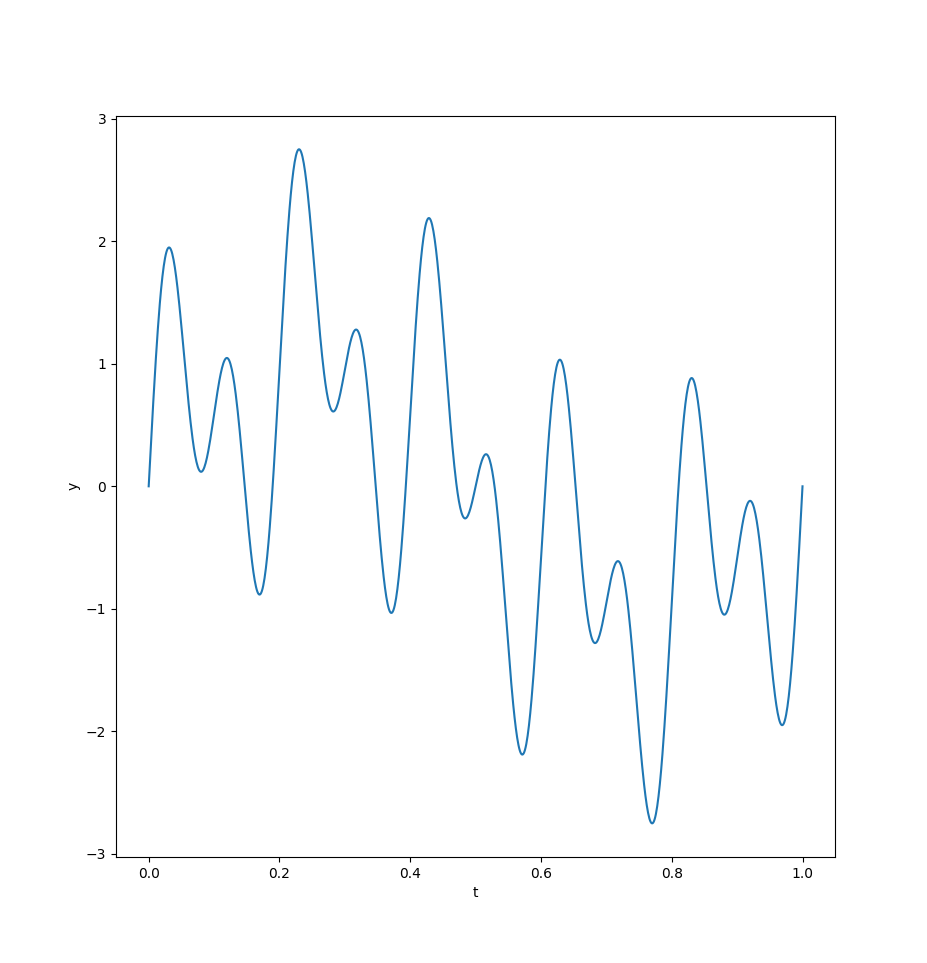
\includegraphics[width=100px]{images/01-what-is-fourier-signal.png}
        \end{column}
        \hspace*{-50px}
        $\rightarrow$
        \begin{column}{60px}
            \centering
            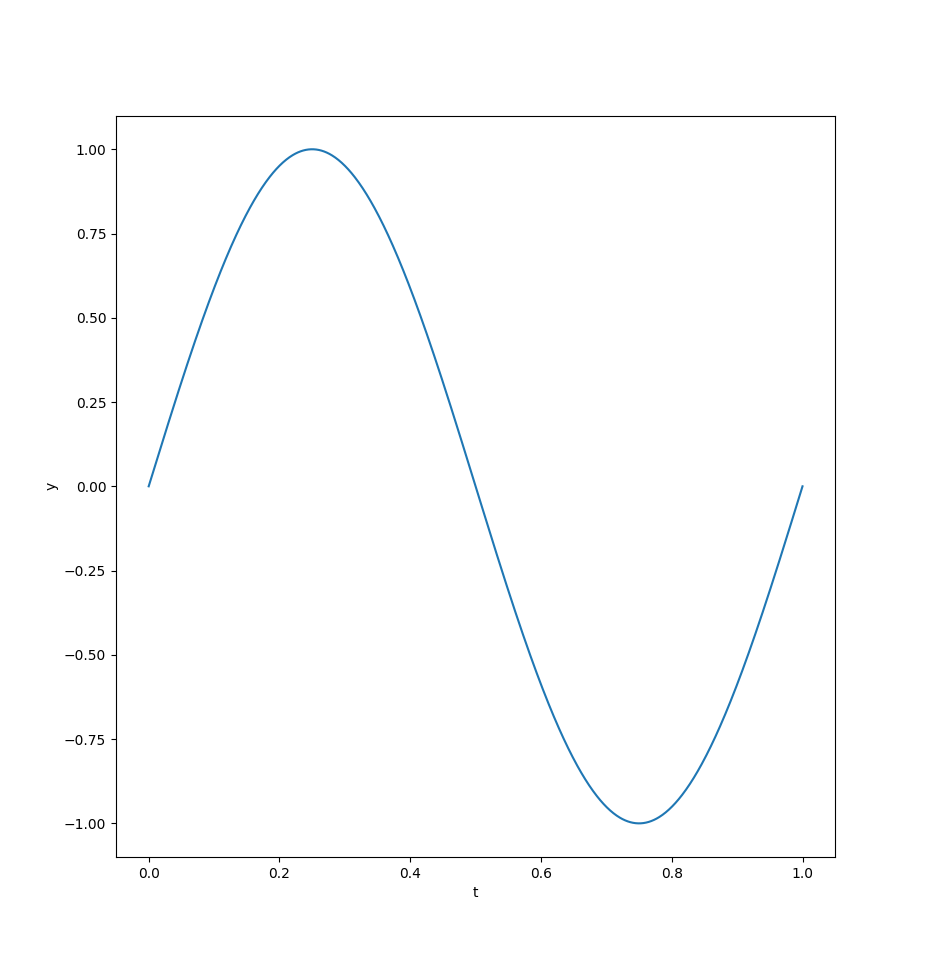
\includegraphics[width=50px]{images/01-what-is-fourier-signal-component-1.png}
            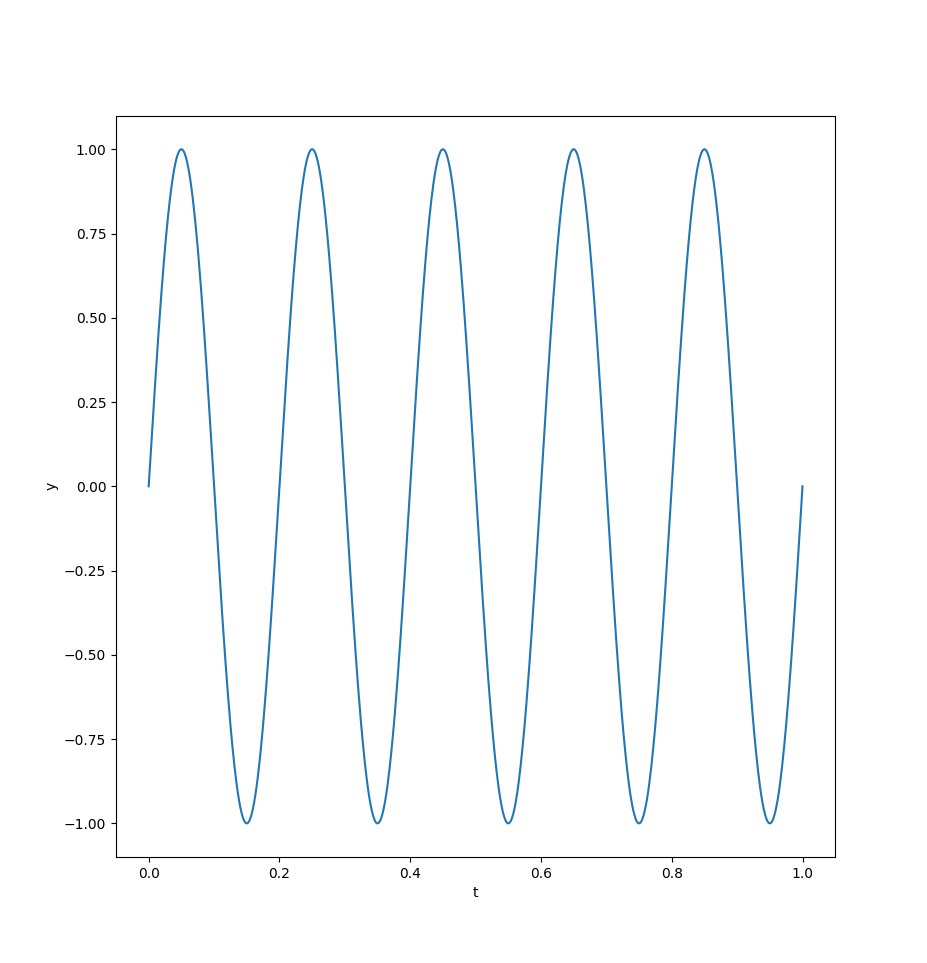
\includegraphics[width=50px]{images/01-what-is-fourier-signal-component-2.png}
            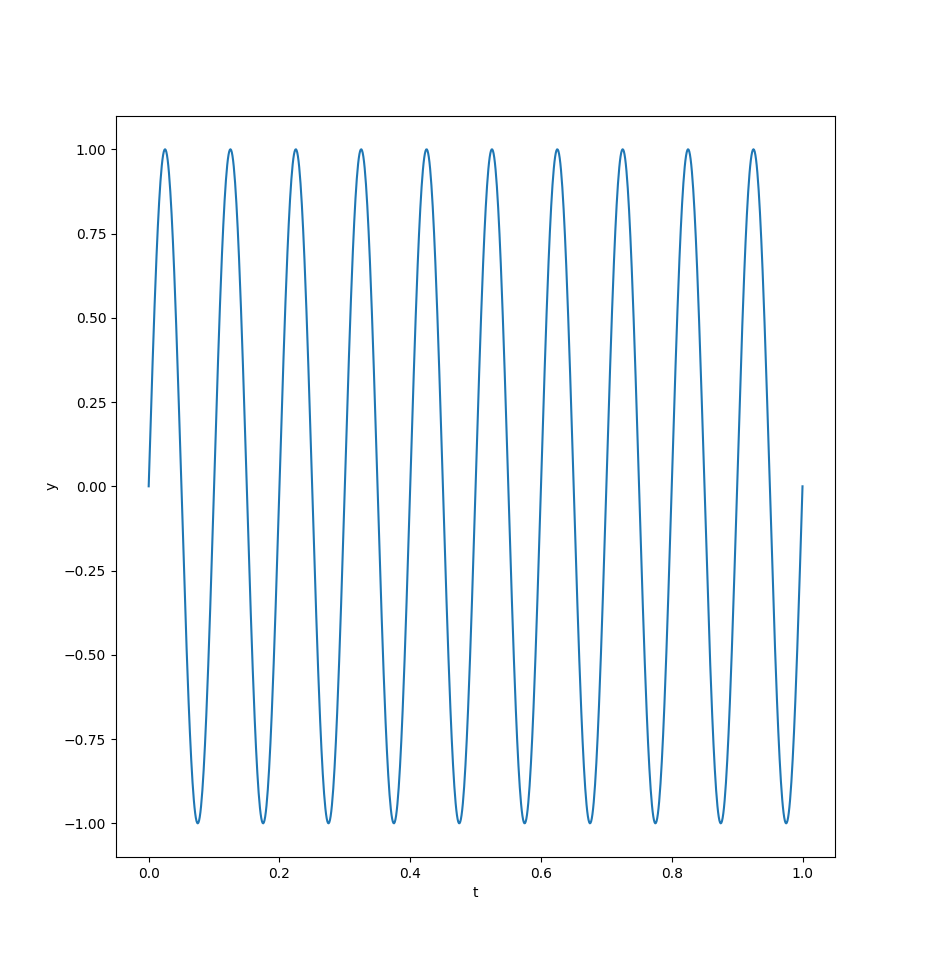
\includegraphics[width=50px]{images/01-what-is-fourier-signal-component-3.png}
        \end{column}
        \hspace*{-40px}
        $\rightarrow$
        \begin{column}{110px}
            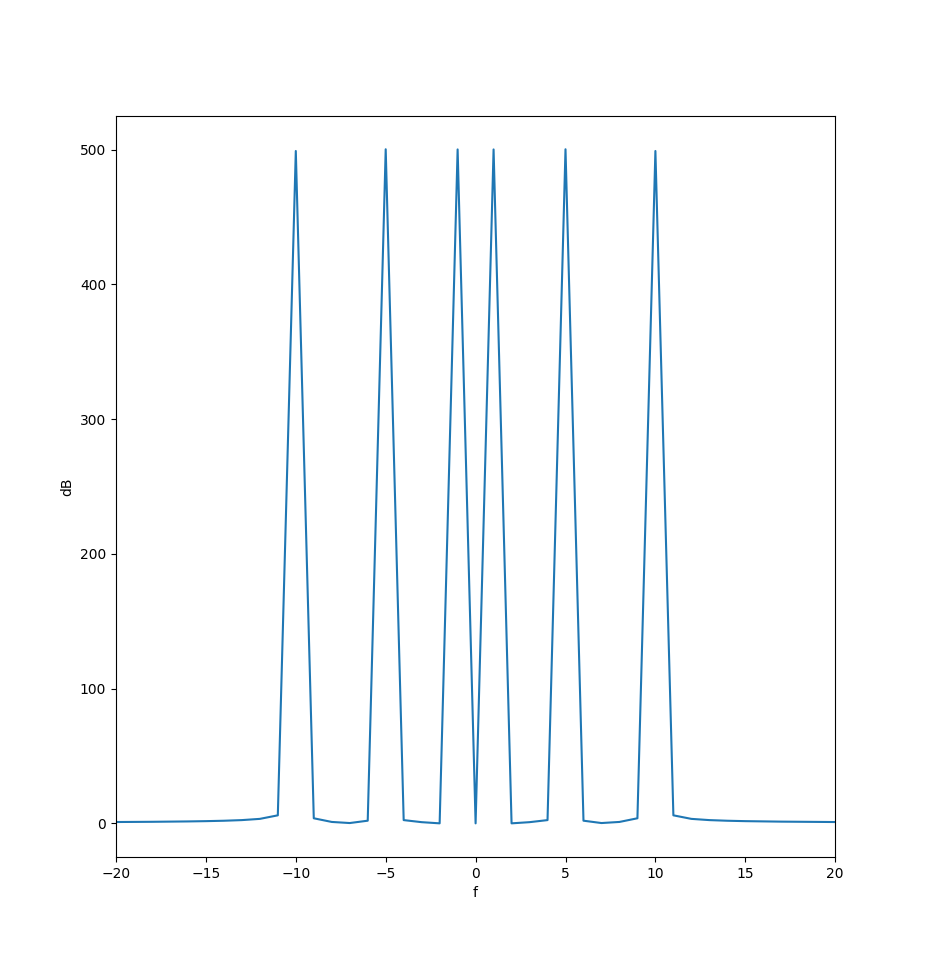
\includegraphics[width=100px]{images/01-what-is-fourier-signal-transform.png}
        \end{column}
    \end{columns}

\end{frame}

    \begin{frame}
    \frametitle{Herleitung der Fourier Transformation} 

    \begin{align*}
        (\mathcal{F} g)(f)=\int_{-\infty}^{\infty}{g(t)\cdot e^{-i2\pi f t}\ dt}
    \end{align*}
\end{frame}

\begin{frame}
    \frametitle{Herleitung der Fourier Transformation}
    \framesubtitle{Eulersche Formel}

    \hspace{-100px}
    \begin{columns}[c]
        \begin{column}{200px}
        \begin{align*}
        e^{i\varphi}=\cos{\varphi}+i\sin{\varphi}
    \end{align*}
\end{column}
\hspace*{-60px}
\begin{column}{100px}
    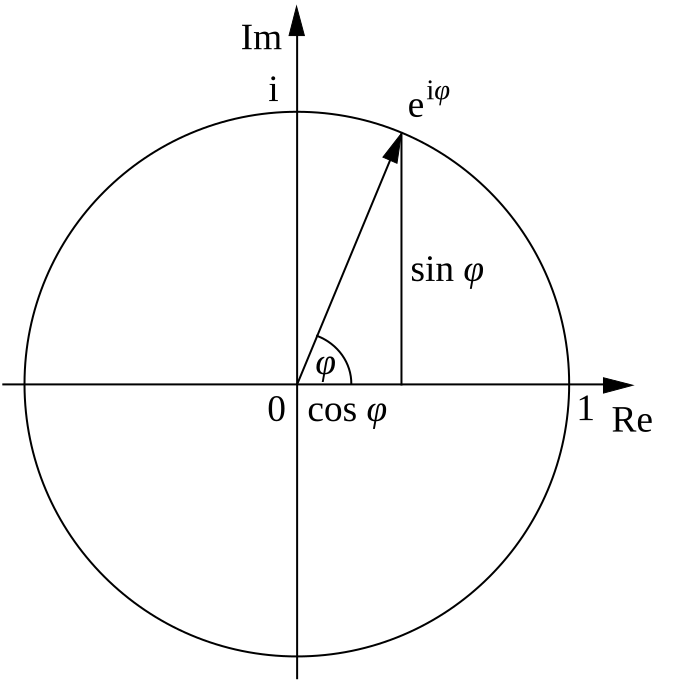
\includegraphics[width=100px]{images/02-deriving-fourier-euler.png}
\end{column}
    \end{columns}
\end{frame}

\begin{frame}
    \frametitle{Herleitung der Fourier Transformation}
    \framesubtitle{Eulersche Formel}

    \hspace{-100px}
    \begin{columns}[c]
        \begin{column}{200px}
        \begin{align*}
        e^{i\varphi}=\cos{\varphi}+i\sin{\varphi}
    \end{align*}
\end{column}
\hspace*{-60px}
\begin{column}{100px}
    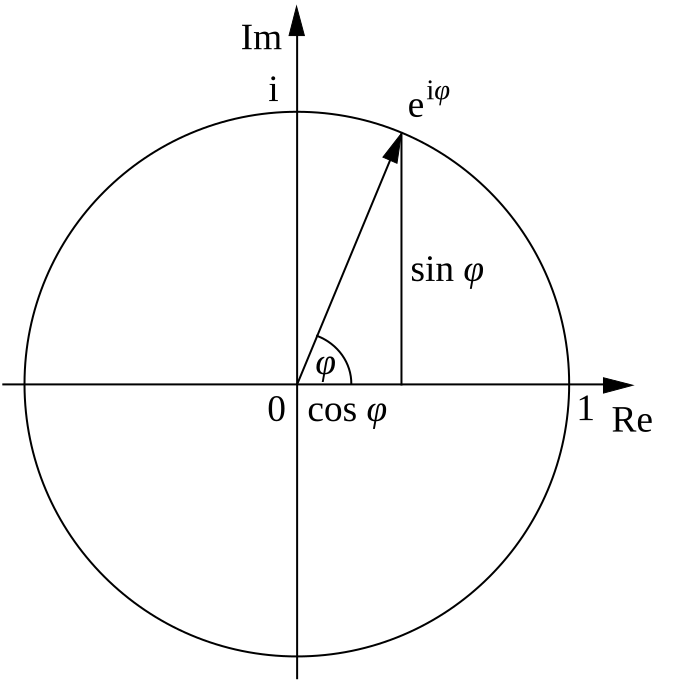
\includegraphics[width=100px]{images/02-deriving-fourier-euler.png}
\end{column}
    \end{columns}
    \vspace{20px}
    Rotieren in der komplexen Ebene mit Frequenz $f$: 
    \begin{align*}
        \varphi&=\omega t=2\pi ft \\
        c(t)&=e^{-i\varphi}\\
            &=e^{-i2\pi f t}
    \end{align*}
\end{frame}

\begin{frame}
    \frametitle{Herleitung der Fourier Transformation}
    \framesubtitle{Rotieren des Signals}

    Signal  $g(t)$ um einen Punkt in der komplexen Ebene rotieren:
    \begin{align*}
        g_c(t, f)=g(t)\cdot e^{-i2\pi f t}
    \end{align*}
    \begin{center}
        \begin{columns}[c]
    \begin{column}{100px}
        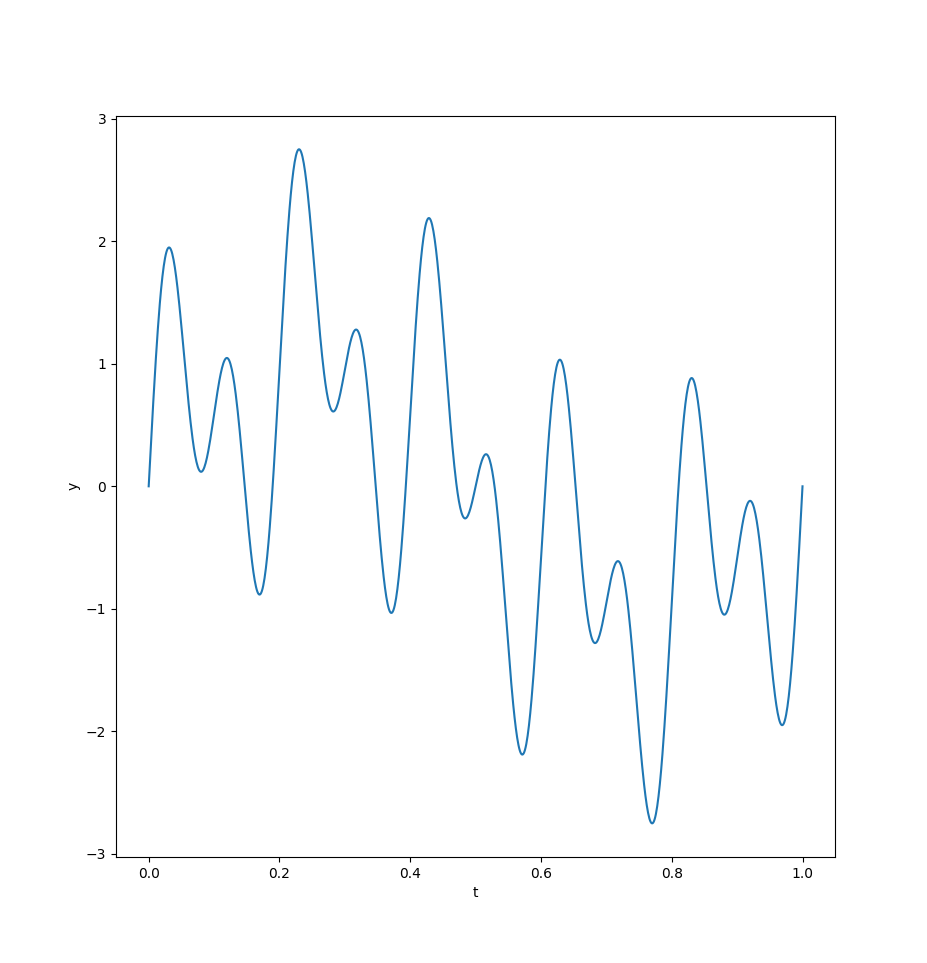
\includegraphics[width=100px]{images/01-what-is-fourier-signal.png}
    \end{column}
    \hspace*{-45px}
    \begin{column}{10px}
        $\overset{\scriptscriptstyle{f=10Hz}}{\parbox{1.1cm}{\rightarrowfill}}$
    \end{column}
    \hspace*{-20px}
    \begin{column}{100px}
        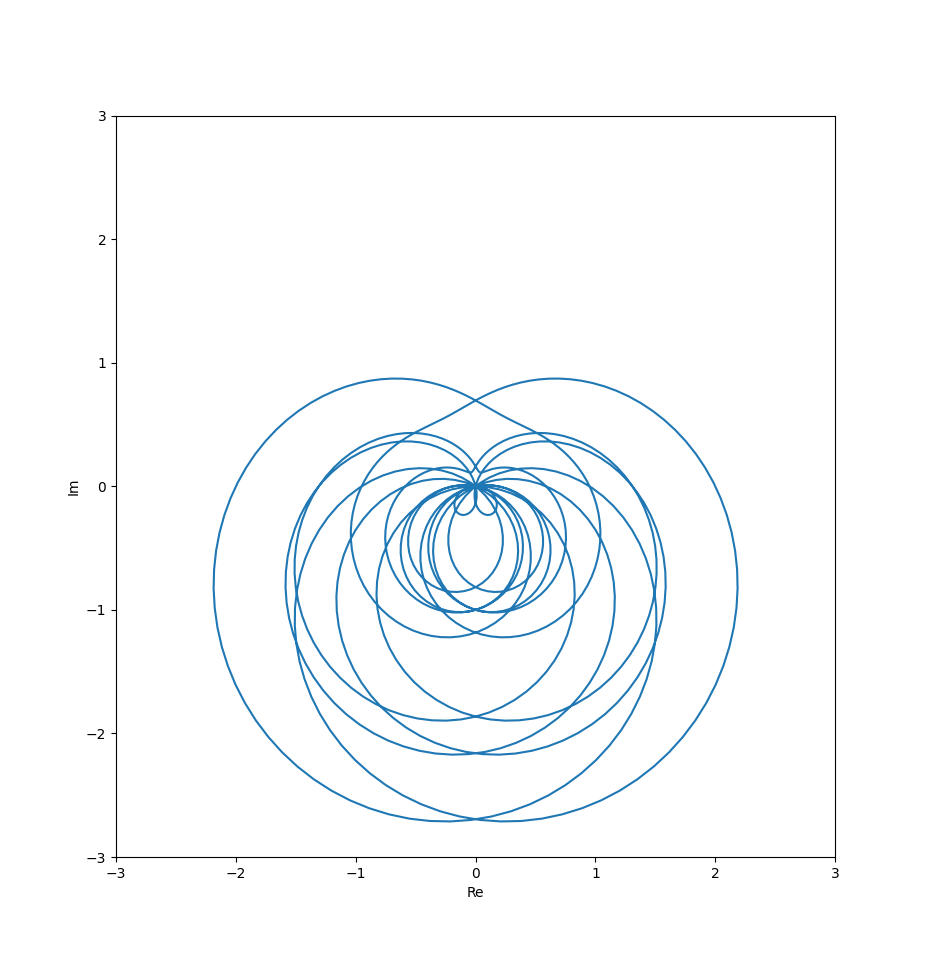
\includegraphics[width=100px]{images/02-deriving-fourier_wrapped_signal.png}
    \end{column}
    \end{columns}
    \end{center}
\end{frame}

\begin{frame}
    \frametitle{Herleitung der Fourier Transformation}
    \framesubtitle{Finden des Durchschnittswertes}
    Durchschnittlichen Wert von $f_c$ finden:
    \begin{align*}
    \frac{1}{N}\cdot \sum_{i=0}^{N}{g(t_i)\cdot e^{-i2\pi f t_i}}
    \end{align*}
    \begin{center}
    $\downarrow$ 
\end{center}
    \begin{align*}
        \frac{1}{t_2-t_1}\cdot \int_{t_1}^{t_2}{g(t)\cdot e^{-i2\pi f t}\ dt}
    \end{align*}
    \begin{itemize}
        \item[?]Entfernen des $\frac{1}{t_2-t_1}$ Terms 
    \end{itemize}
\end{frame}

\begin{frame}
    \frametitle{Herleitung der Fourier Transformation}
    \framesubtitle{Finden des Durchschnittswertes}
    Durchschnittlichen Wert von $f_c$ finden:
    \begin{align*}
        \frac{1}{t_2-t_1}\cdot \int_{t_1}^{t_2}{g(t)\cdot e^{-i2\pi f t}\ dt}
    \end{align*}
    \frametitle{Herleitung der Fourier Transformation}
    Entfernen des $\frac{1}{t_2-t_1}$ Terms:
    \begin{align*}
    \int_{t_1}^{t_2}{g(t)\cdot e^{-i2\pi f t}\ dt}
    \end{align*}
    \begin{itemize}
        \item Wenn eine Frequenz lange im Signal auftaucht, wird der Peak höher
    \end{itemize}
\end{frame}

\begin{frame}
    \frametitle{Herleitung der Fourier Transformation}
    Erweitern der Integrationsgrenzen:
    \begin{align*}
        \int_{-\infty}^{\infty}{g(t)\cdot e^{-i2\pi f t}\ dt}=(\mathcal{F}g)(f)
    \end{align*}

    \vspace{10px}
    \begin{tcolorbox}[colback=red!5!white,colframe=red!75!black,title=Wichtig]
        $(\mathcal{F} g):\mathbb{R}\rightarrow\mathbb{C}$ ist die komplexwertige Fourier Transformation\newline
        $\abs{(\mathcal{F} g)(f)}\ $ beschreibt die Anwesenheit von Frequenz $f$\newline
         $\angle (\mathcal{F} g)(f)\ $ ist die Phasenverschiebung von Frequenz $f$
    \end{tcolorbox}
\end{frame}

    
\begin{frame}
    \frametitle{Inverse Fourier Transformation}
    \begin{columns}
        \begin{column}{80px}
            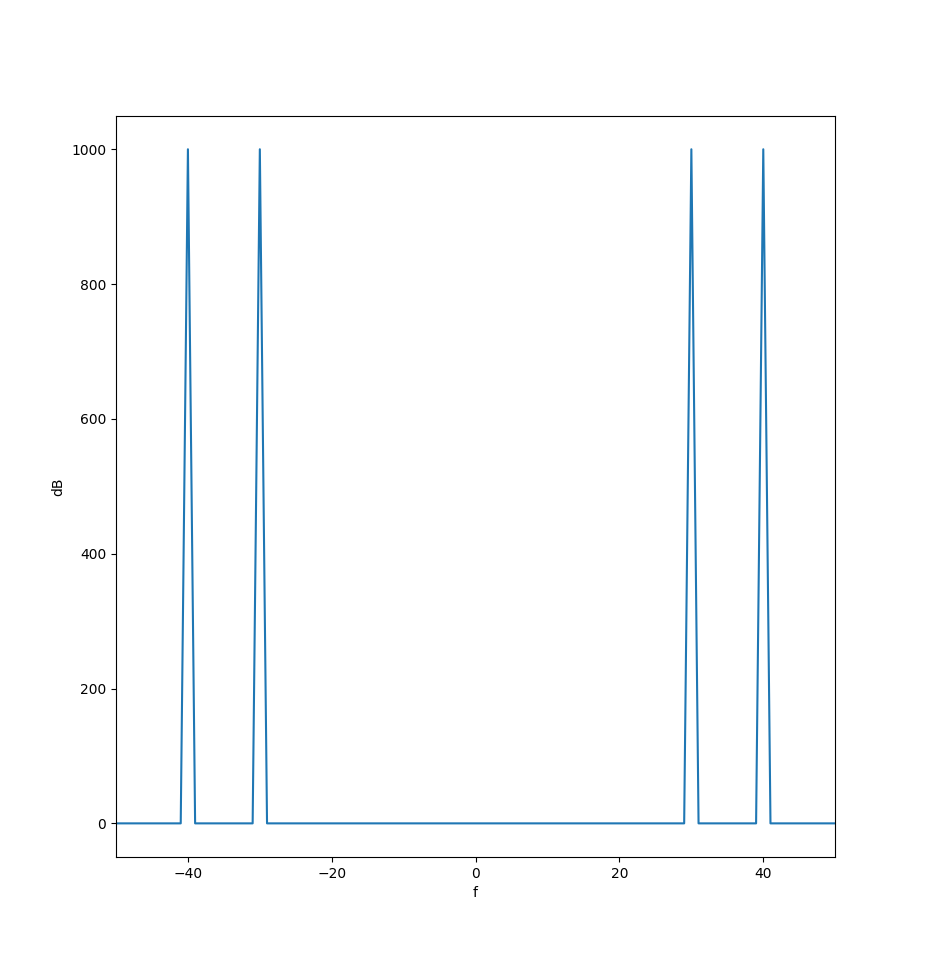
\includegraphics[width=80px, caption=Magnitude]{images/03-ift-mag.png} 
            \centering
            +
            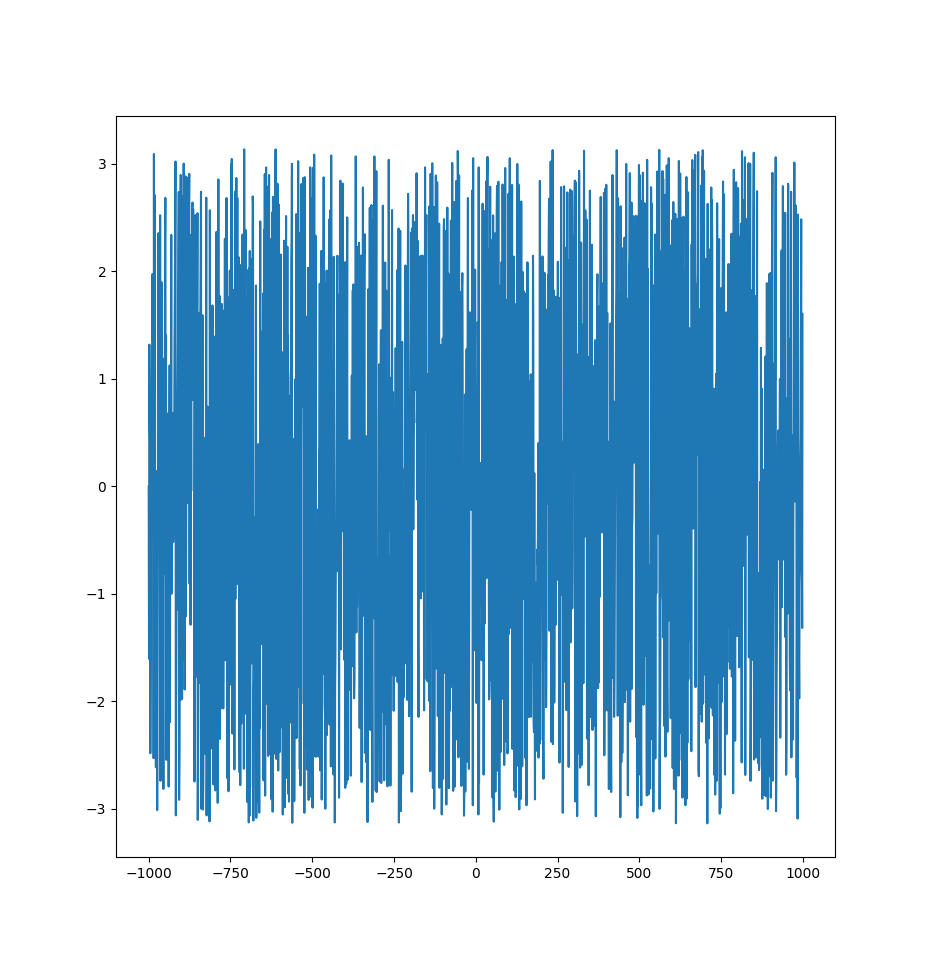
\includegraphics[width=80px]{images/03-ift-phase.png}
        \end{column}
        \hspace*{-40px}
        \begin{column}{5px}
            =
        \end{column}
        \hspace*{-40px}
        \begin{column}{100px}
            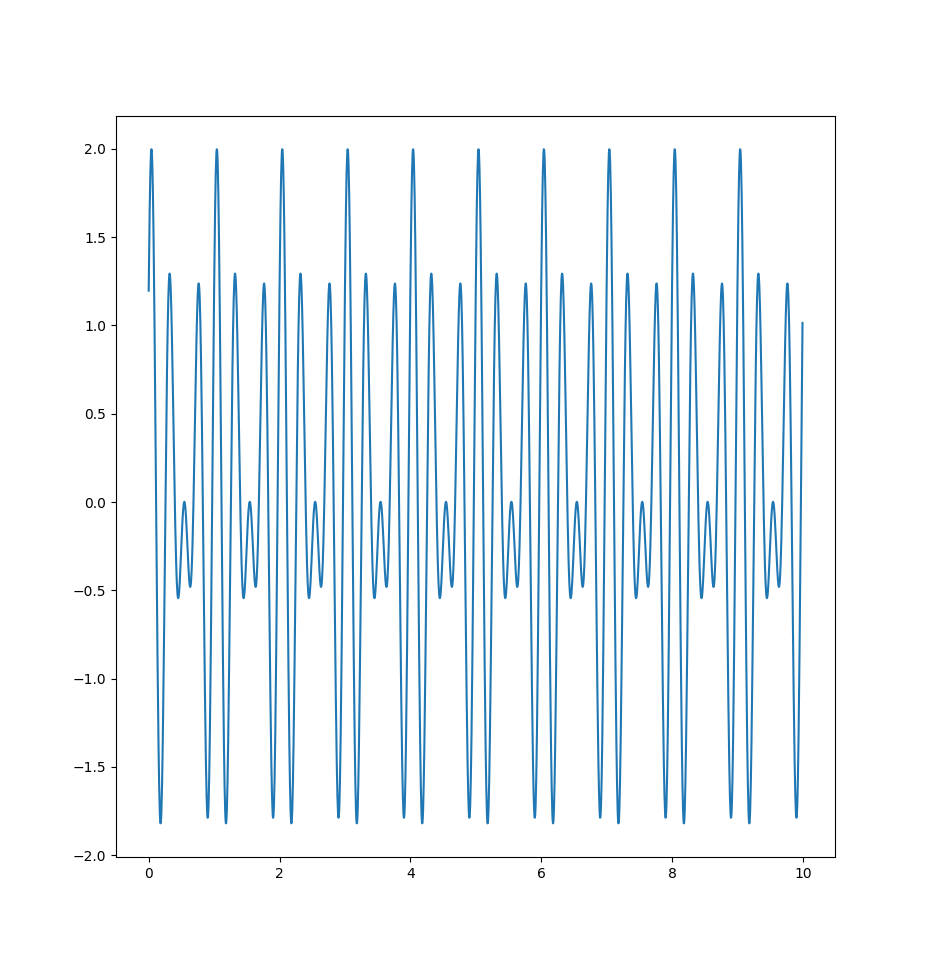
\includegraphics[width=100px]{images/03-ift-reconstructed.png} 
        \end{column}

    \end{columns}
\end{frame}

\begin{frame}
    \frametitle{Inverse Fourier Transformation}
    \begin{align*}
        g(t)=\int_{-\infty}^{\infty}{(\mathcal F g)(f)\cdot  e^{i2\pi f t}\ df}
    \end{align*} 
    \begin{itemize}
        \item Zwischen beiden Transformationen gehen keine Informationen verloren
    \end{itemize}
    \begin{align*}
        \Rightarrow \mathcal{F}^{-1}(\mathcal F g)(f)=g(x)
    \end{align*}
    \vspace*{-15px}
    \begin{itemize}
        \item[?] Wofür wird diese Rücktransformation benutzt
    \end{itemize}
\end{frame}

\begin{frame}
    \frametitle{Inverse Fourier Transformation}
    \begin{align*}
        g(t)=\int_{-\infty}^{\infty}{(\mathcal F g)(f)\cdot  e^{i2\pi f t}\ df}
    \end{align*} 
    \begin{itemize}
        \item Zwischen beiden Transformationen gehen keine Informationen verloren
    \end{itemize}
    \begin{align*}
        \Rightarrow \mathcal{F}^{-1}(\mathcal F g)(f)=g(x)
    \end{align*}
    \vspace*{-15px}
    \begin{itemize}
        \item Besonders nützlich z.B. für das Filtern von Frequenzen
    \end{itemize}
\end{frame}

    \begin{frame}
	\frametitle{Diskrete Fourier Transformation}
	\begin{itemize}
		\item Fourier Transformation ist ein mathematisches Verfahren um Frequenzen von kontinuierlichen Signalen zu erhalten
		\item Computer arbeiten nur mit diskreten Werten
		\item Wie können zeitdiskrete Signale in ihre Frequenzen zerlegt werden?
	\end{itemize}
\end{frame}

\begin{frame}
	\frametitle{Diskrete Fourier Transformation}
	\begin{align*}
		c_k &= \sum_{n=0}^{N-1}s_n e^{-i2\pi k n / N}
	\end{align*}
	\begin{itemize}
		\item N = Anzahl an Samples
		\item $s_n$ = Sample n
		\item k = Frequenz aus $[0,N-1]$
		\item $c_k$ = DFT mit Information zu Amplitude und Phase
	\end{itemize}
\end{frame}

\begin{frame}
	\frametitle{Inverse DFT}
	\begin{align*}
		s_n &= \frac{1}{N} \sum_{k=0}^{N-1}c_k e^{i2\pi k n/N}
	\end{align*}
\end{frame}
    \begin{frame}
    \frametitle{Audioverarbeitung}
    \framesubtitle{Spektrogramm}
    Visualisierung von Signalen in einem Spektrogramm:
    \begin{itemize}
        \item Visualisiert den zeitlichen Verlauf des Frequenzspektrums
        \item Für jeden Zeitpunkt eine Fourier Analyse
        \item Signalanalyse, Musikerkennung
    \end{itemize} 
    \begin{columns}
        \begin{column}{120px}
            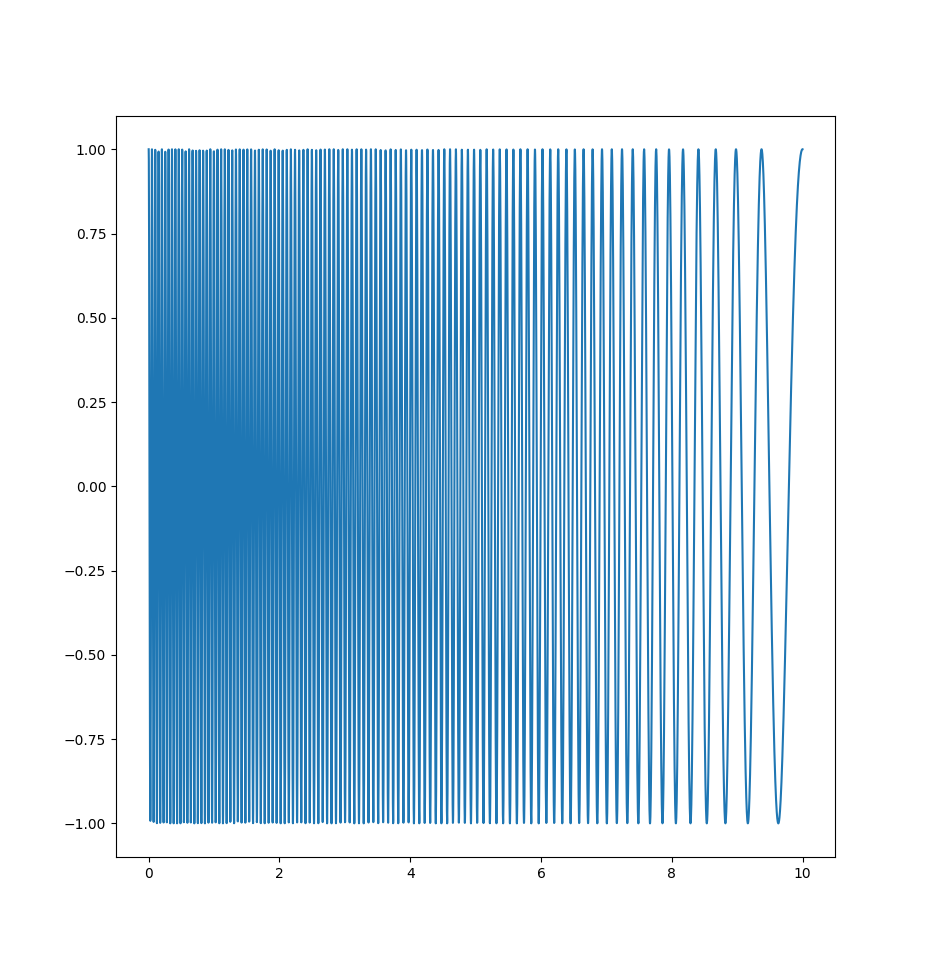
\includegraphics[width=120px]{images/04-applications-audio-chirp.png}
        \end{column}
        \hspace*{-25px}
        \begin{column}{5px}
            $\rightarrow$
        \end{column}
        \hspace*{-25px}
        \begin{column}{120px}
            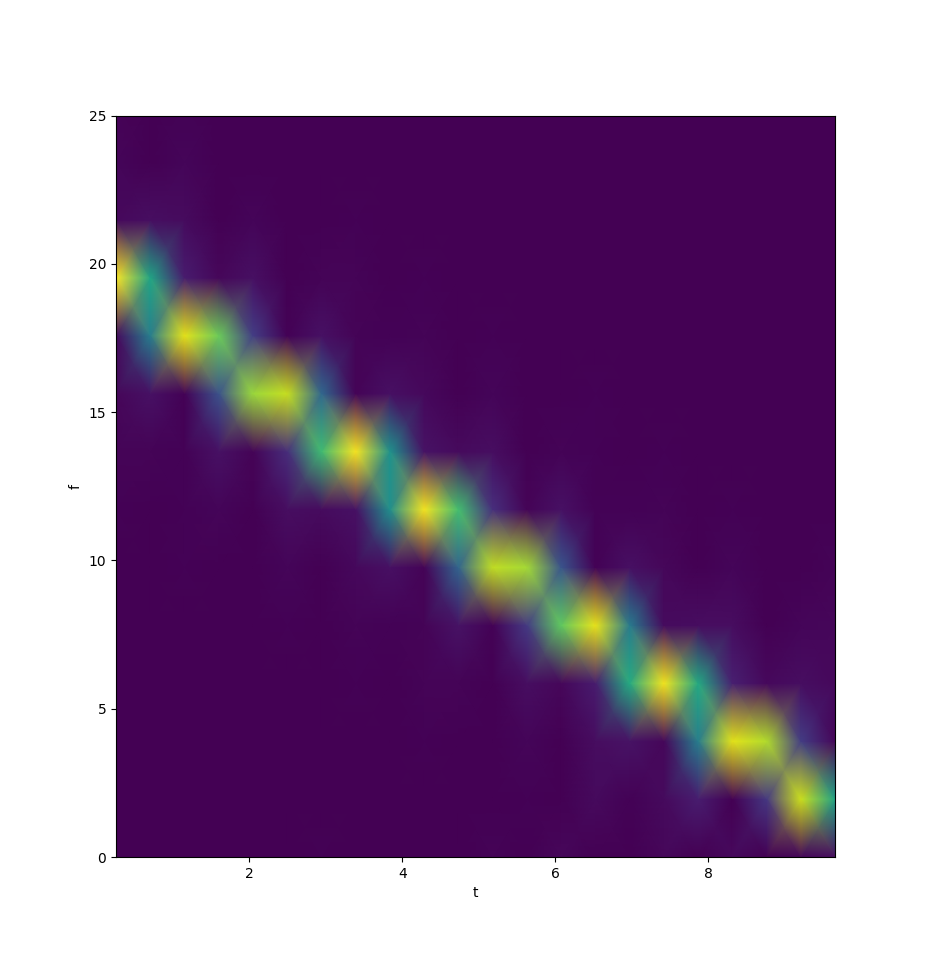
\includegraphics[width=120px]{images/04-applications-audio-chirp-spectrogram.png} 
        \end{column}
    \end{columns}
\end{frame}

\begin{frame}
    \frametitle{Audioverarbeitung}
    \framesubtitle{Frequenzfilterung}
    Filtern von Frequenzen:
    \begin{itemize}
        \item Identifizieren von Störfrequenzen
        \item Eliminierung von diesem aus Frequenzspektrum
        \item Inverse Fourier Transformation anwenden
    \end{itemize}
\end{frame}

\begin{frame}
    \frametitle{Anwendungen}
    \framesubtitle{Audio}

    \begin{columns}
        \begin{column}{160px}
            \centering
            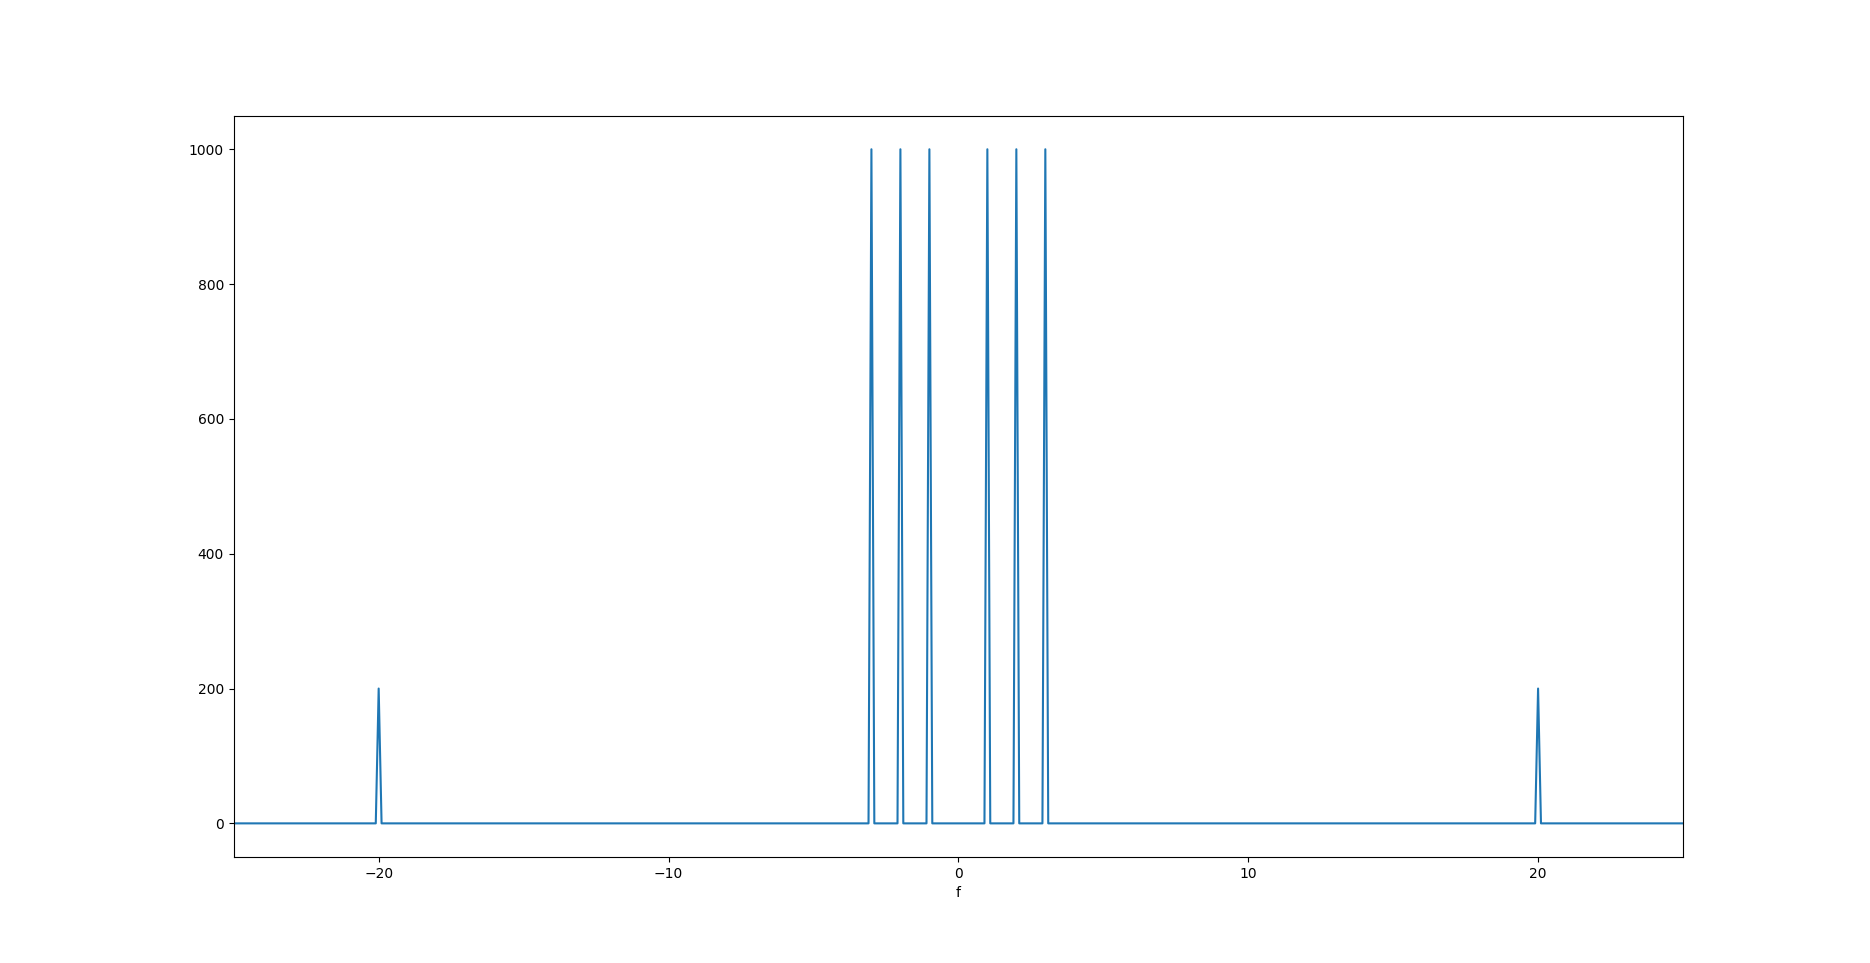
\includegraphics[width=160px]{images/04-applications-audio-noisy-signal-ft.png}
            $\downarrow$
            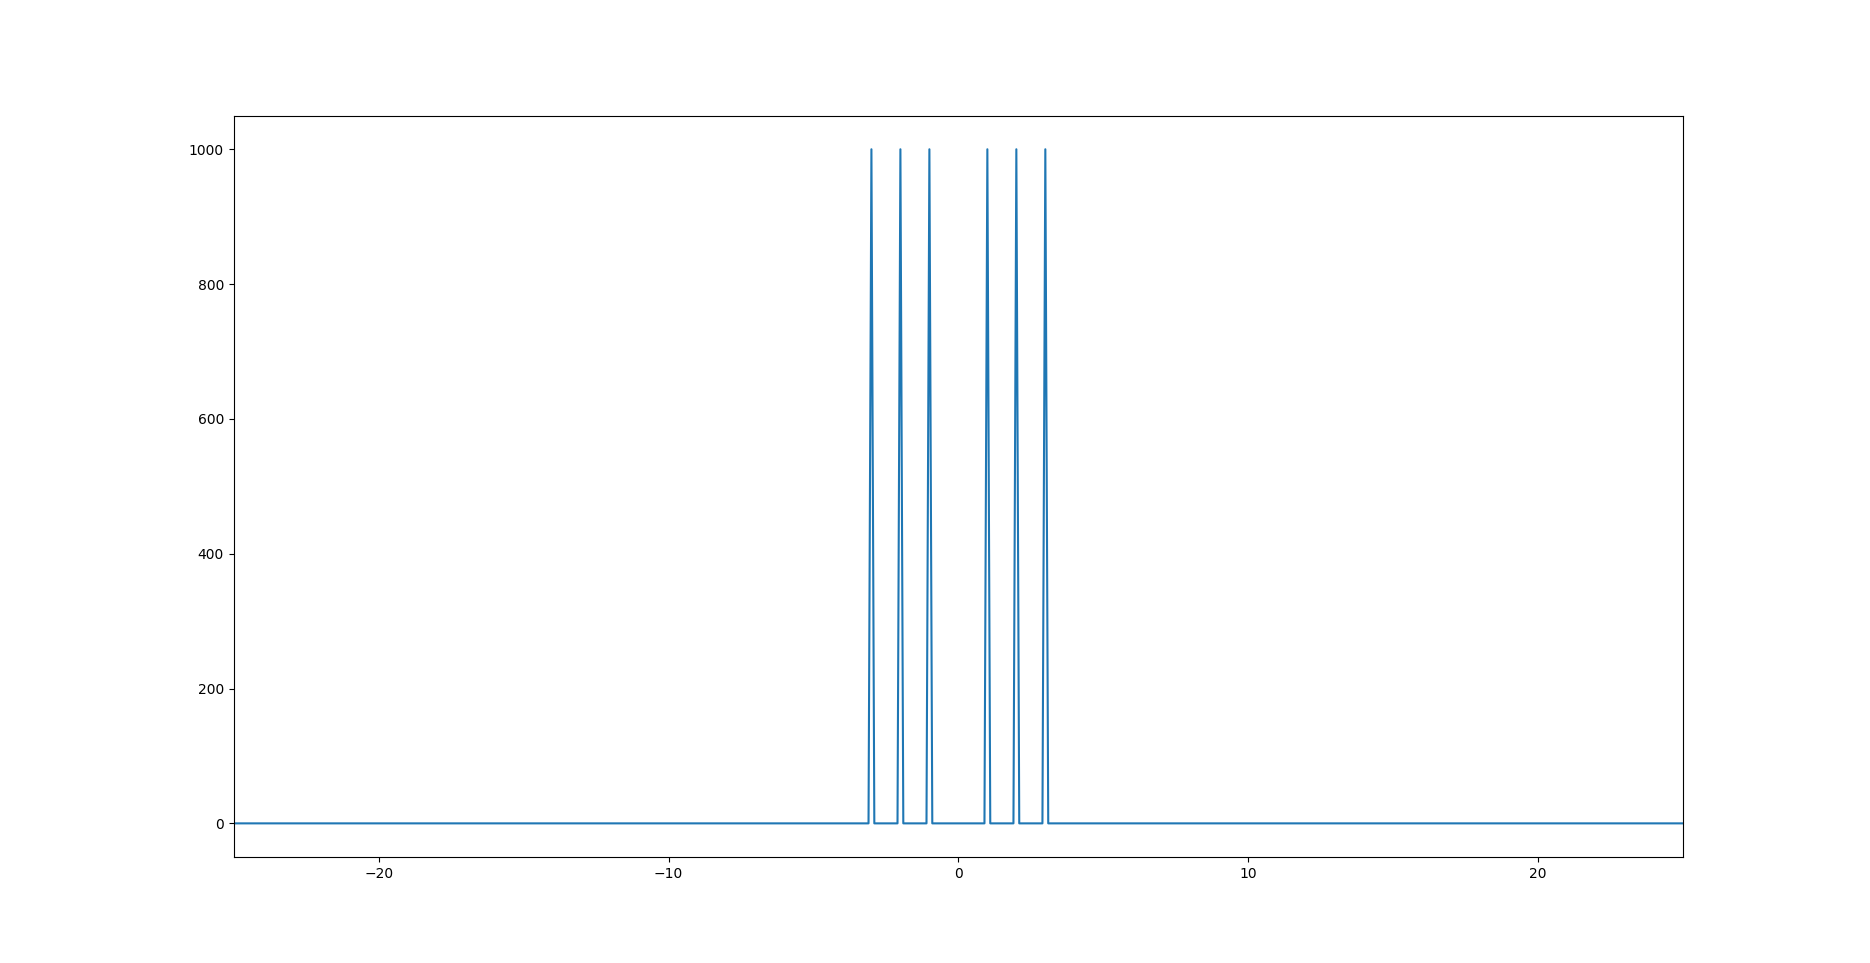
\includegraphics[width=160px]{images/04-applications-audio-clean-signal-ft.png}
        \end{column}
        \hspace*{-25px}
        \begin{column}{1px}
            \vspace*{-13px}
            \begin{align*}
                \overset{FT}\longleftarrow \\ \\ \\ \\ \\ \\
                \overset{IFT}\longrightarrow
            \end{align*}
        \end{column}
        \hspace*{-25px}
        \begin{column}{100px}
            \centering
            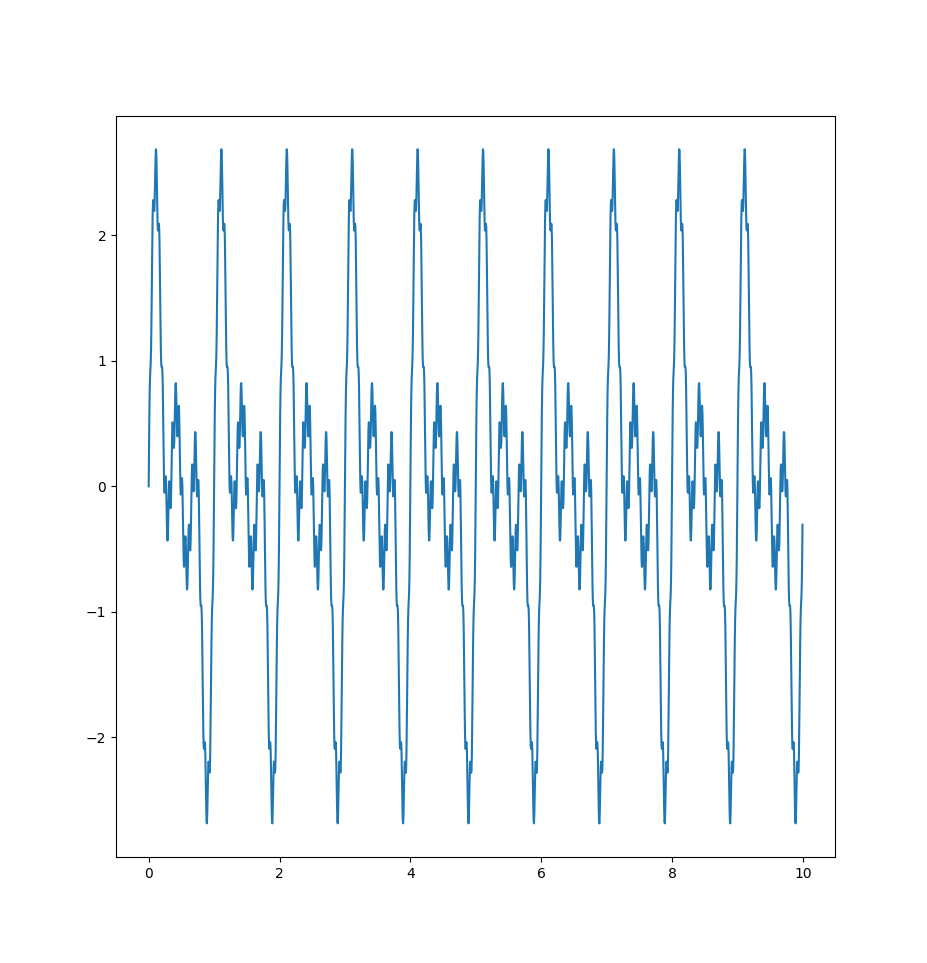
\includegraphics[width=100px]{images/04-applications-audio-noisy-signal.png}
            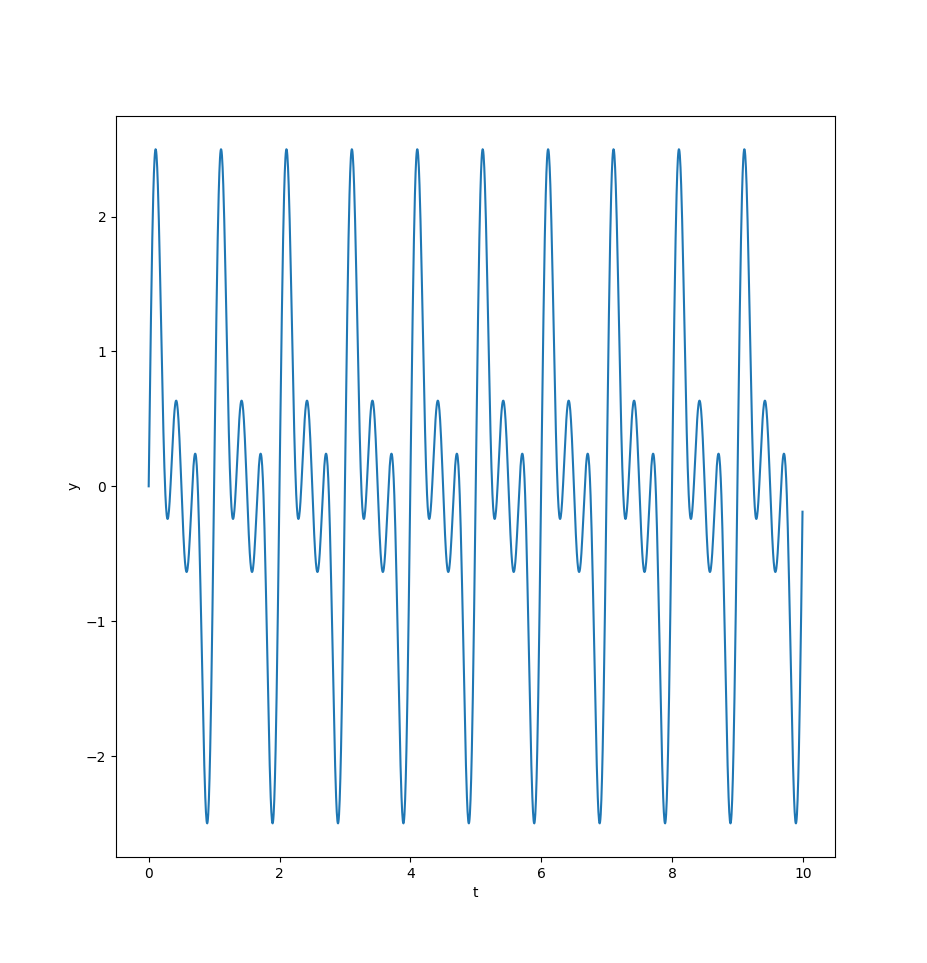
\includegraphics[width=100px]{images/04-applications-audio-clean-signal-ift.png}
        \end{column}
    \end{columns}
\end{frame}

\begin{frame}
    \frametitle{Bildverarbeitung}
    \framesubtitle{Voraussetzungen}

    \begin{itemize}
        \item Benötigt eine 2-Dimensionale Fourier Transformation
    \end{itemize}
    \begin{align*}
        (\mathcal{F} b)(k, l)=\int_{-\infty}^{\infty}{\int_{-\infty}^{\infty}{b(x, y)\cdot e^{-i2\pi (kx+ly)} \ dx}\ dy}
    \end{align*}
    Oder diskret:
    \begin{align*}
        (\mathcal{F} b)(k, l)=\sum_{x=0}^{X-1}{\sum_{y=0}^{Y-1}{b(x,y)\cdot e^{-i(\omega_kx+\omega_ly)}}}
    \end{align*}
\end{frame}

\begin{frame}
    \frametitle{Bildverarbeitung}
    \framesubtitle{Eigenschaften der 2D-FT}

    \begin{itemize}
        \item Der Fourier Raum hat die gleiche Dimension wie das Bild
        \item x-Achse und y-Achse beschreiben Frequenzen
        \item Die Farbe eines Pixels beschreibt die Magnitude/Phase
        \item Punktsymmetrisch um den Ursprung
    \end{itemize}
\end{frame}

\begin{frame}
    \frametitle{Bildverarbeitung}
    \framesubtitle{2D Fourier Raum}
    \centering
    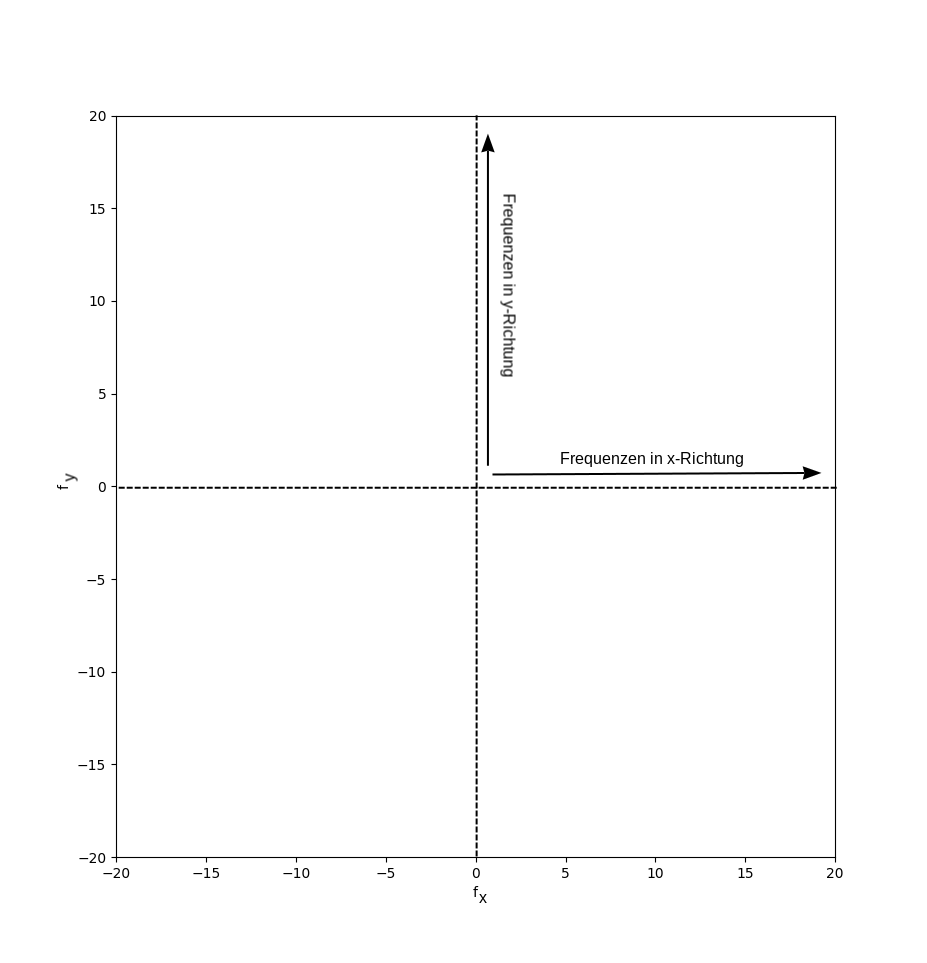
\includegraphics[width=170px]{images/04-applications-fourier-space-empty.png}
\end{frame}

\begin{frame}
    \frametitle{Bildverarbeitung}
    \framesubtitle{2D Fourier Raum}
    \centering
    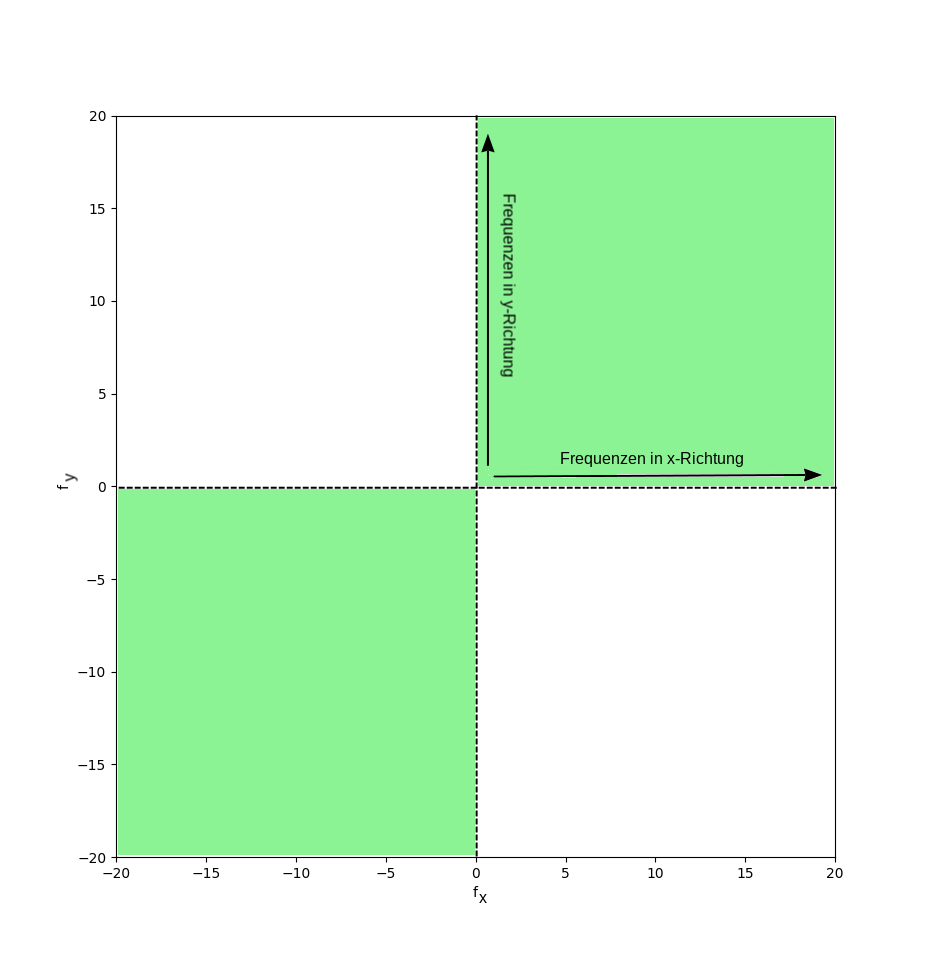
\includegraphics[width=170px]{images/04-applications-fourier-space-empty-1.png}
\end{frame}

\begin{frame}
    \frametitle{Bildverarbeitung}
    \framesubtitle{2D Fourier Raum}
    \centering
    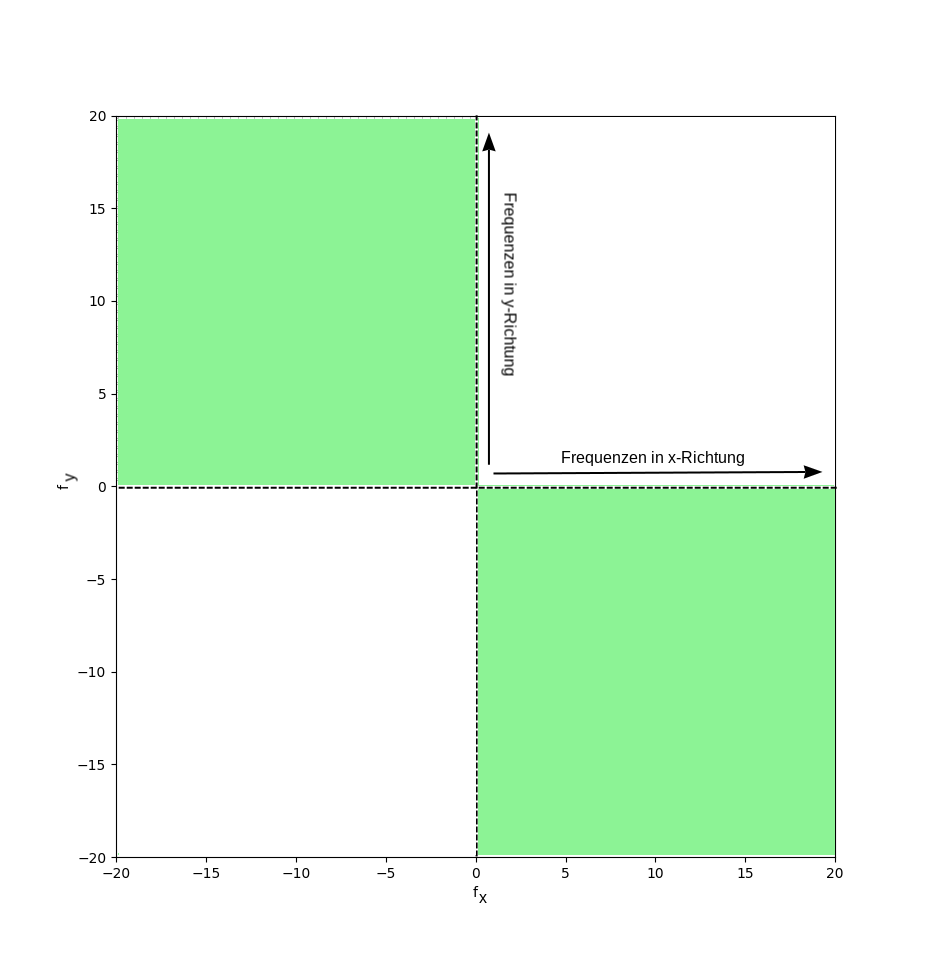
\includegraphics[width=170px]{images/04-applications-fourier-space-empty-2.png}
\end{frame}

\begin{frame}
    \frametitle{Bildverarbeitung}
    \framesubtitle{Fourier Transformation von einfachen Kosinusbildern}
    \begin{columns}
        \begin{column}{100px}
            \centering
            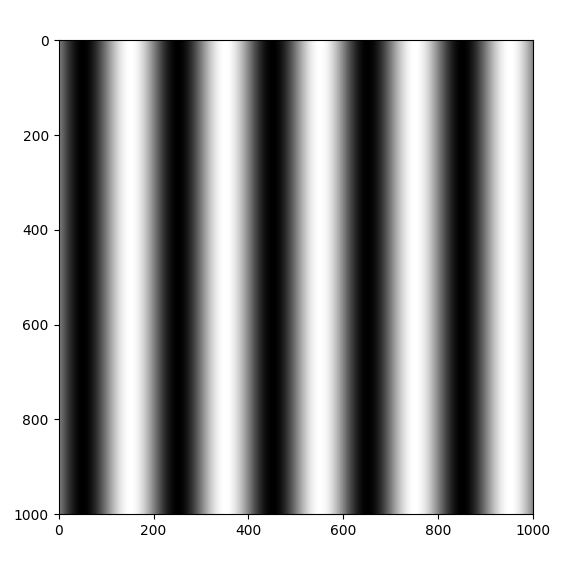
\includegraphics[width=100px]{images/04-applications-image-cos.png}
            $\downarrow$
            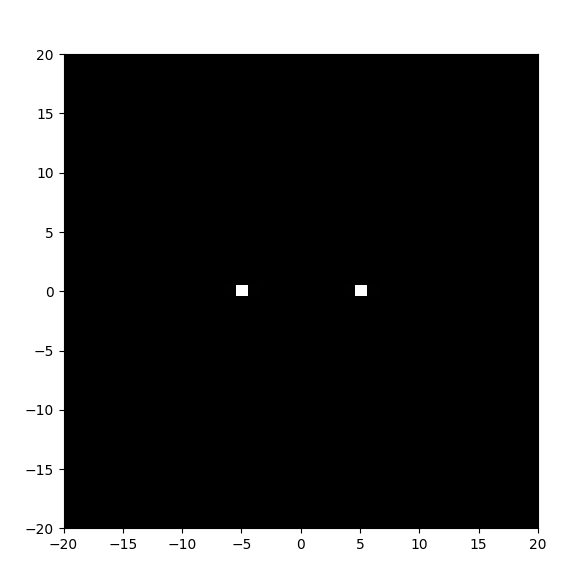
\includegraphics[width=100px]{images/04-applications-image-cos-ft.png}
        \end{column}
    \end{columns}
\end{frame}

\begin{frame}
    \frametitle{Bildverarbeitung}
    \framesubtitle{Fourier Transformation von einfachen Kosinusbildern}
    \begin{columns}
        \begin{column}{100px}
            \centering
            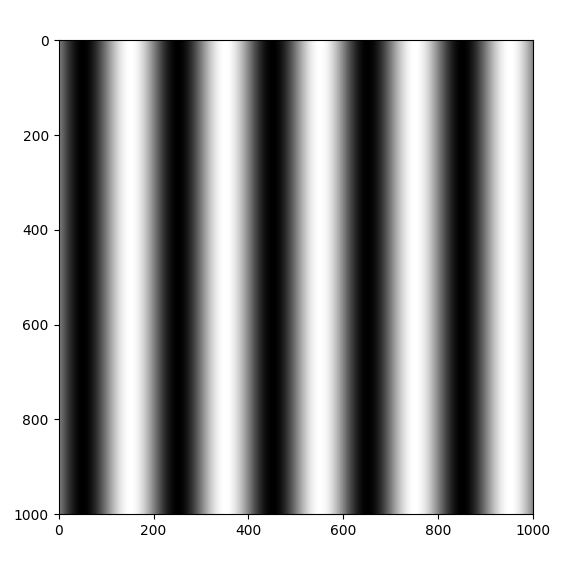
\includegraphics[width=100px]{images/04-applications-image-cos.png}
            $\downarrow$
            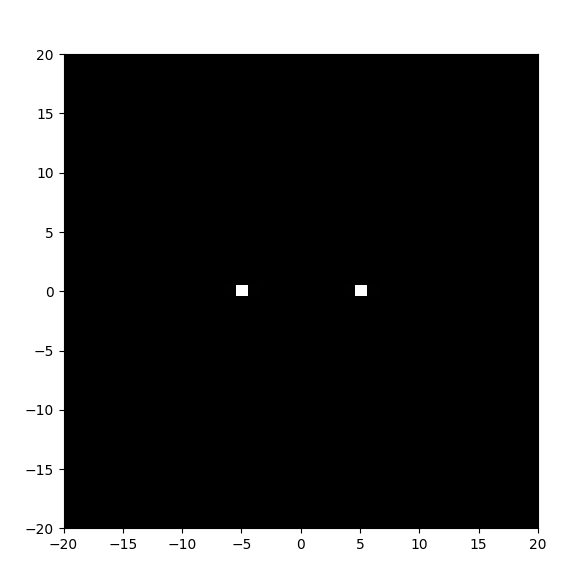
\includegraphics[width=100px]{images/04-applications-image-cos-ft.png}
        \end{column}
        \begin{column}{100px}
            \centering
            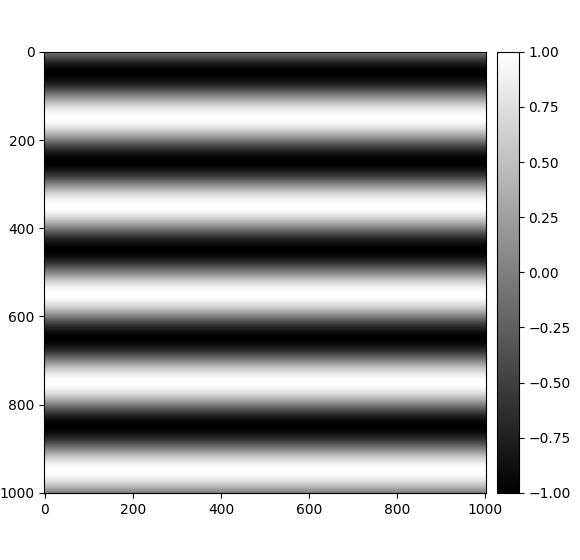
\includegraphics[width=100px]{images/04-applications-image-cos-rot.png}
            $\downarrow$
            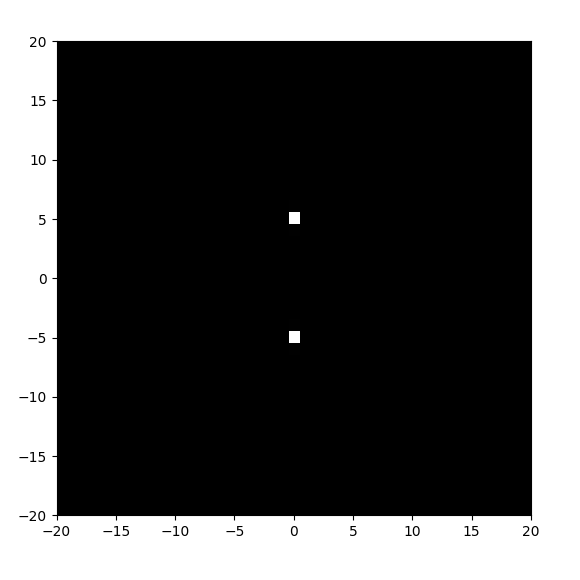
\includegraphics[width=100px]{images/04-applications-image-cos-rot-ft.png}
        \end{column}
    \end{columns}
\end{frame}

\begin{frame}
    \frametitle{Bildverarbeitung}
    \framesubtitle{Fourier Transformation von einfachen Kosinusbildern}
    \begin{columns}[t]
        \begin{column}{100px}
            \centering
            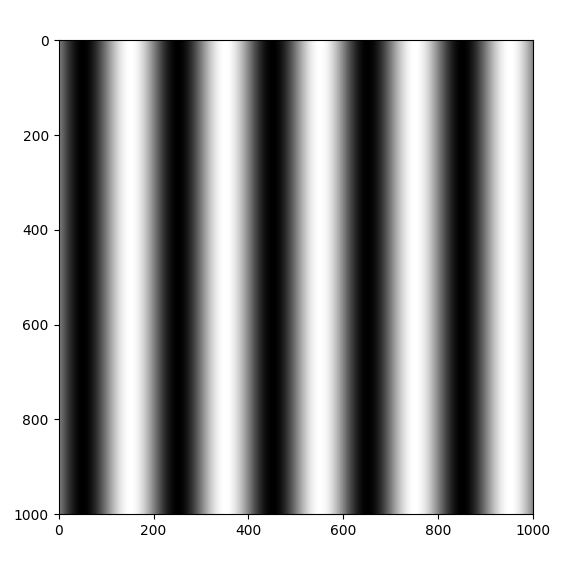
\includegraphics[width=100px]{images/04-applications-image-cos.png}
            \downarrow
            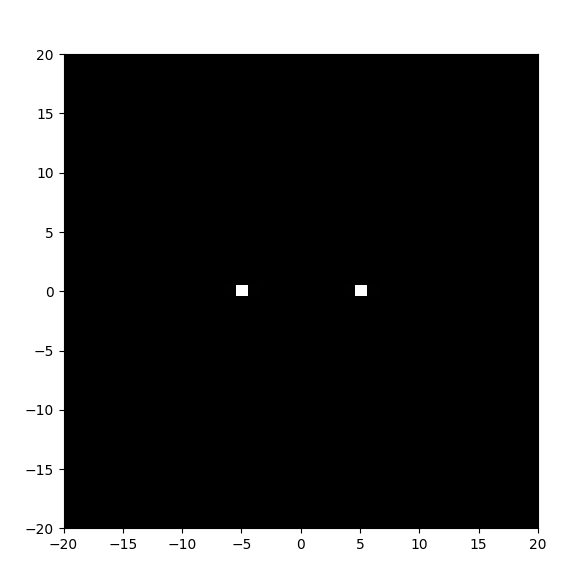
\includegraphics[width=100px]{images/04-applications-image-cos-ft.png}
        \end{column}
        \begin{column}{100px}
            \centering
            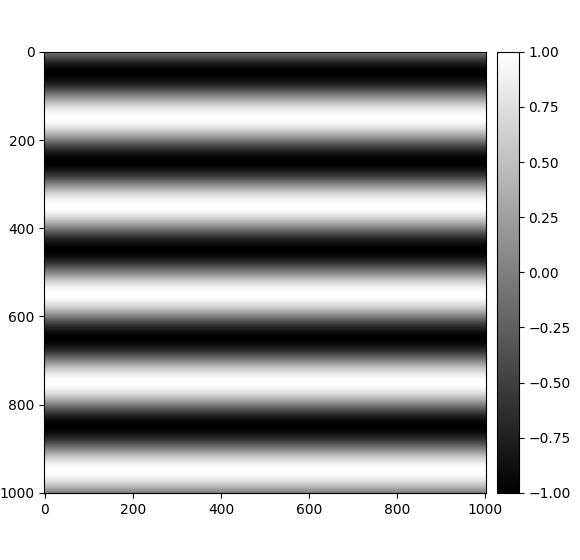
\includegraphics[width=100px]{images/04-applications-image-cos-rot.png}
            \downarrow
            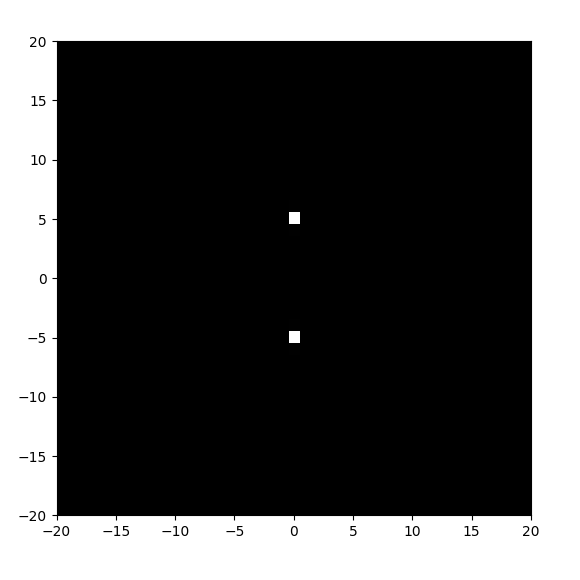
\includegraphics[width=100px]{images/04-applications-image-cos-rot-ft.png}
        \end{column}
        \begin{column}{100px}
            \centering
            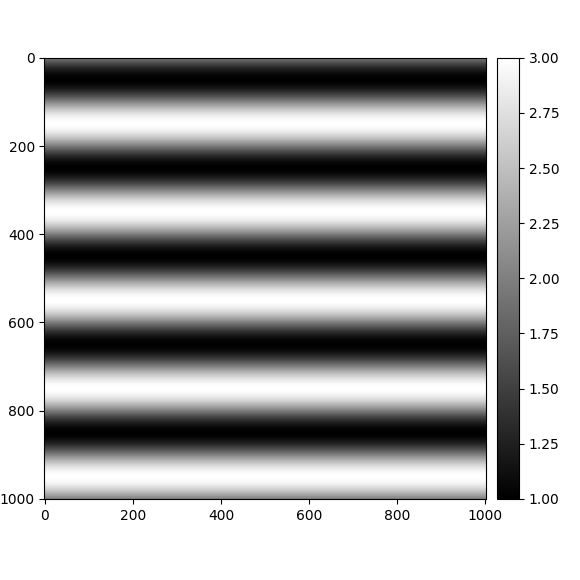
\includegraphics[width=100px]{images/04-applications-image-cos-rot-dc.png}
        \begin{tcolorbox}[halign=center, colback=white, boxrule=0pt, colframe=white, enlarge top by=-0.45cm]
            $\downarrow$ 

            \vspace{30px}
            \LARGE{?}
            \end{tcolorbox}
        \end{column}
    \end{columns}
\end{frame}

\begin{frame}
    \frametitle{Bildverarbeitung}
    \framesubtitle{Fourier Transformation von einfachen Kosinusbildern}
    \begin{columns}
        \begin{column}{100px}
            \centering
            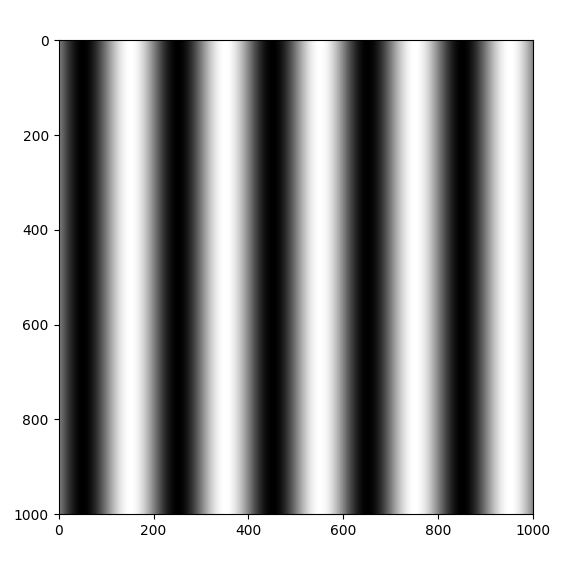
\includegraphics[width=100px]{images/04-applications-image-cos.png}
            $\downarrow$
            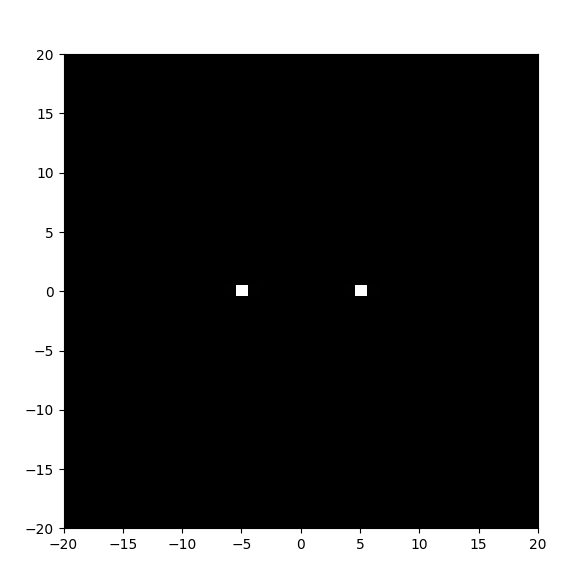
\includegraphics[width=100px]{images/04-applications-image-cos-ft.png}
        \end{column}
        \begin{column}{100px}
            \centering
            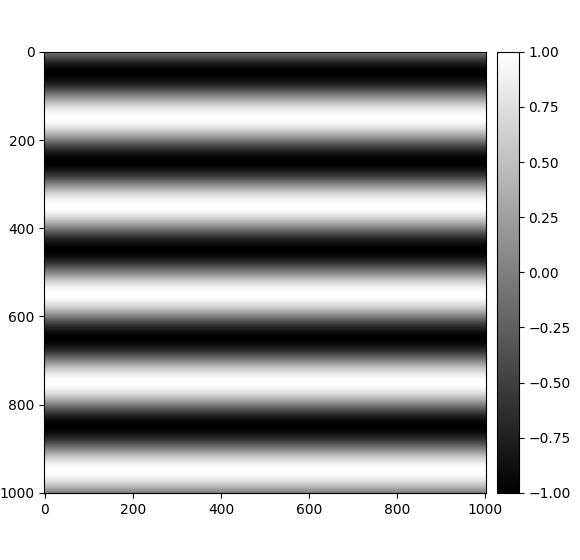
\includegraphics[width=100px]{images/04-applications-image-cos-rot.png}
            $\downarrow$
            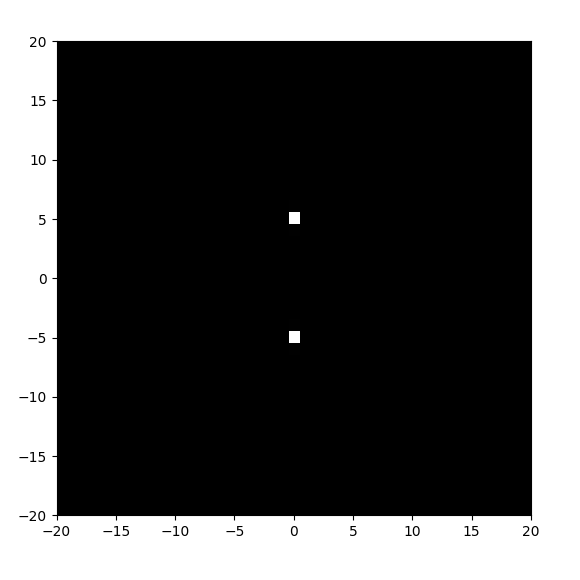
\includegraphics[width=100px]{images/04-applications-image-cos-rot-ft.png}
        \end{column}
        \begin{column}{100px}
            \centering
            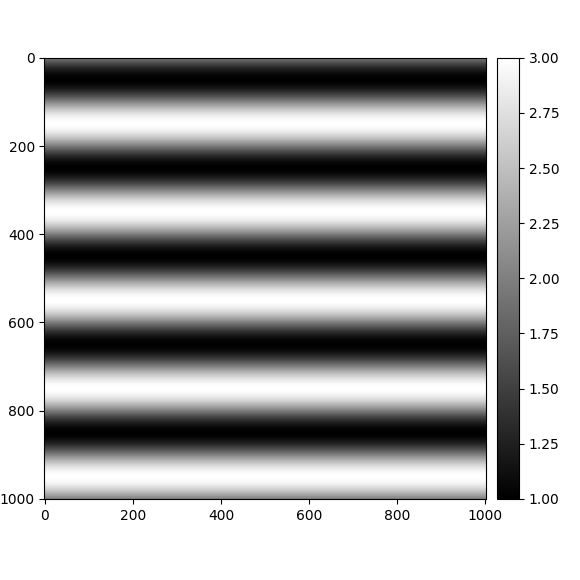
\includegraphics[width=100px]{images/04-applications-image-cos-rot-dc.png}
            $\downarrow$
            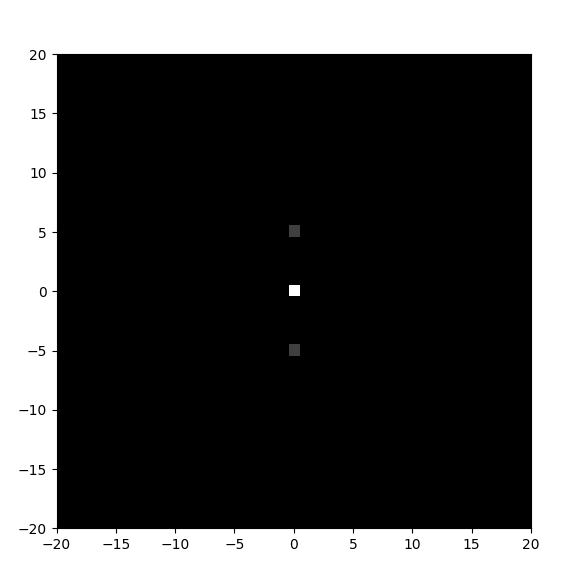
\includegraphics[width=100px]{images/04-applications-image-cos-rot-dc-ft.png}
        \end{column}
    \end{columns}
\end{frame}

\begin{frame}
    \frametitle{Bildverarbeitung}
    \framesubtitle{Schräge Kosinusbilder}
    Schräger Kosinus:
    \begin{itemize}
        \item Kanteneffekte wenn nicht periodisch
    \end{itemize}
    \begin{columns}
        \begin{column}{100px}   
            \includegraphics[width=100px]{images/04-applications-image-cos-rot-45-0.png}
        \end{column} 
        \hspace*{-30px}
        \begin{column}{5px}
            $\rightarrow$
        \end{column}
        \hspace*{-30px}
        \begin{column}{120px}
            \includegraphics[width=120px]{images/04-applications-image-cos-rot-45-0-ft.png}
        \end{column}
    \end{columns}
\end{frame}

\begin{frame}
    \frametitle{Bildverarbeitung}
    \framesubtitle{Schräge Kosinusbilder}

    \begin{itemize}
        \item Die Fouriertransformation nimmt das Signal als periodisch weitergeführt an
    \end{itemize}

    \vspace{10px}
    \centering
    \includegraphics[width=100px]{images/04-applications-image-rot-45.png}

    \vspace{5px}
    \begin{itemize}
        \item Starke Kanten
        \item Hohe diagonale Frequenzen
    \end{itemize}
\end{frame}

\begin{frame}
    \frametitle{Bildverarbeitung}
    \framesubtitle{Kanten}
    \begin{itemize}
        \item Scharfe Kanten sind mit Frequenzbändern im Fourier Raum verbunden        
        \item Für jede Kante ein Frequenzband
    \end{itemize}
    \begin{columns}
        \begin{column}{100px}
            \includegraphics[width=100px]{images/04-applications-image-cubes.jpg}
        \end{column}
        \hspace*{-50px}
        \begin{column}{5px}
            $\rightarrow$
        \end{column}
        \hspace*{-50px}
        \begin{column}{100px}
            \includegraphics[width=100px]{images/04-applications-image-cubes-ft.png}
        \end{column}
    \end{columns}
\end{frame}

\begin{frame}
    \frametitle{Bildverarbeitung}
    \framesubtitle{Hochpass}
    \begin{itemize}
        \item Filtert niedrige Frequenzen aus dem Bild heraus
    \end{itemize}
    \begin{columns}[c]
        \begin{column}{90px}
            \centering
            \includegraphics[width=90px]{images/04-applications-image-lena-ft.png}
            $\downarrow$
            \includegraphics[width=90px]{images/04-applications-image-lena-ft-high-pass-ft.png}
        \end{column}
        \hspace*{-35px}
        \begin{column}{1px}
            \vspace*{-13px}
            \begin{align*}
                \overset{FT}\longleftarrow \\ \\ \\ \\ \\ \\
                \overset{IFT}\longrightarrow
            \end{align*}
        \end{column}
        \hspace*{-35px}
        \begin{column}{100px}
            \centering
            \includegraphics[width=70px]{images/04-applications-image-lena.png}
            \vspace*{-30px}
            \includegraphics[width=90px]{images/04-applications-image-lena-ft-high-pass.png}
        \end{column}
    \end{columns}
\end{frame}

\begin{frame}
    \frametitle{Bildverarbeitung}
    \framesubtitle{Rauschfilterung}
    \begin{itemize}
        \item Simplifiziertes Beispiel mit nur einer Rauschfrequenz
    \end{itemize}
    \begin{columns}
        \begin{column}{120px}
            \includegraphics[width=120px]{images/04-applications-image-lena-cos.png} 
        \end{column}    
        \hspace*{-30px}
        \begin{column}{5px}
            $\overset{FT}{\longrightarrow}$
        \end{column}
        \hspace*{-30px}
        \begin{column}{120px}
            \includegraphics[width=120px]{images/04-applications-image-lena-cos-ft.png}
        \end{column}
    \end{columns}
\end{frame}

\begin{frame}
    \frametitle{Bildverarbeitung}
    \framesubtitle{Rauschfilterung}

    \begin{itemize}
        \item Rauschfrequenz aus Spektrum entfernen
    \end{itemize}

    \begin{columns}
        \begin{column}{120px}
            \includegraphics[width=120px]{images/04-applications-image-lena-cos-ft-fixed.png} 
        \end{column}    
        \hspace*{-30px}
        \begin{column}{5px}
            $\overset{FT}{\longrightarrow}$
        \end{column}
        \hspace*{-30px}
        \begin{column}{120px}
            \includegraphics[width=120px]{images/04-applications-image-lena-cos-fixed.png}
        \end{column}
    \end{columns}
\end{frame}

    
\end{document}

